\documentclass{beamer}
\usetheme{}
\usecolortheme{dolphin}           
\useinnertheme{circles}
\setbeamertemplate{itemize items}[default]
\setbeamertemplate{enumerate items}[default]
\usepackage[T1]{fontenc}
\usepackage[utf8]{inputenc}
\usepackage{lmodern}
\usepackage{amsmath}
\usepackage{booktabs} 
\usepackage{graphicx}        
\usepackage{array}
\usepackage{color}
\usepackage{textcomp}
\usepackage{epstopdf}                     % For EPS figures
\makeatletter
\def\zapcolorreset{\let\reset@color\relax\ignorespaces}
\def\colorrows#1{\noalign{\aftergroup\zapcolorreset#1}\ignorespaces}
\makeatother
\graphicspath{{/home/swl/Dropbox/ucd/international_trade/tex/}} 
\setbeamertemplate{navigation symbols}{}

%--------------------------------------
%%%% DETAILS TITLE PAGE %%%%
%--------------------------------------
\title{Specific factors model}
\author{School of Economics, University College Dublin}
\date{Autumn 2017}
\begin{document}
%--------------------------------------
%%%% TITLE SLIDE %%%%
%--------------------------------------
\begin{frame}
\titlepage  
\end{frame}

%--------------------------------------
\begin{frame}
  Last lecture we discussed comparative advantage which entails that some countries have an advantage in the production of particular goods due to lower opportunity costs
  \begin{itemize}
    \item These are due to technological differences which means that there are potential gains to be made from free trade
  \end{itemize}
  \medskip
  In the Ricardian model countries will focus their production on the good in which they have a comparative advantage
  \begin{itemize}
    \item Full specialisation will occur under the free trade equilibrium
  \end{itemize}
  \medskip
  The main insight of this model is that free trade will benefit all participants, even if some countries are terrible at everything
  \begin{itemize}
    \item All workers gain since all income goes to labour
  \end{itemize}
\end{frame}
%--------------------------------------

%--------------------------------------
\begin{frame}
  Despite the useful insights it provides, the Ricardian model has two main shortcomings relating to the predictions it generates
  \medskip  
    \begin{enumerate}
      \item Full specialisation rarely happens
      \item Everyone is expected to benefit from trade since there is only one production factor      
    \end{enumerate}
\end{frame}
%--------------------------------------


%--------------------------------------
\begin{frame}
  Recall that the law of comparative advantage establishes a relationship between trade flows and relative autarky prices
  \begin{align*}
    \frac{p_x}{py} > \frac{p_x^*}{p_y^*}
  \end{align*}
  It is unclear however in the Ricardian framework where these autarky prices come from.
\end{frame}
%--------------------------------------

%--------------------------------------
\begin{frame}
  \textbf{Factor proportion theory} provides a solution as we do know that countries differ in
  \medskip
  \begin{enumerate}
    \item Factor abundance or the relative factor supply
    \item Factor intensity or the relative factor demand
  \end{enumerate}
  \medskip 
  The interaction between factor abundance and intensity determines relative prices and thus trade patterns.  
  We will be discussing two models relying on this concept
  \begin{enumerate}
    \item Specific factors 
    \item Heckscher-Ohlin
  \end{enumerate}
  \medskip
  Factor proportion theory can help us better understand who benefits from trade.
\end{frame}
%--------------------------------------

%--------------------------------------
\begin{frame}
  Let's go back to the prediction of the Ricardian model that trade will be beneficial for all. 
  This ignores the effect of trade on within-country income distribution as trade affects income because
  \medskip
  \begin{enumerate}
    \item Industries differ in production factors that they use
    \begin{itemize}
      \item Stolper-Samuelson Theorem
    \end{itemize}
    \item Production factors cannot move instantly and without costs between industries
  \end{enumerate}
\end{frame}
%--------------------------------------

%--------------------------------------
\begin{frame}
  \textbf{Stolper-Samuelson theorem}   
  \begin{quote}
    Under constant returns to scale, an increase in the price of a commodity will increase the return to the factor used intensively in the production of the commodity and decrease the return to other factors.
  \end{quote}
  \medskip
  We will discuss into more detail next lecture.
\end{frame}
%--------------------------------------

%--------------------------------------
\begin{frame}
  Besides benefits there are also costs associated with opening up to trade, or reducing trade barriers.
  There are costs in the 
  \medskip  
  \begin{enumerate}
    \item short run, such as adjustment costs
    \item long run, due to decrease in the requirement of certain production factors
  \end{enumerate}
\end{frame}
%--------------------------------------

%--------------------------------------
\begin{frame}{source: The Wall Street Journal}
  \begin{figure}
    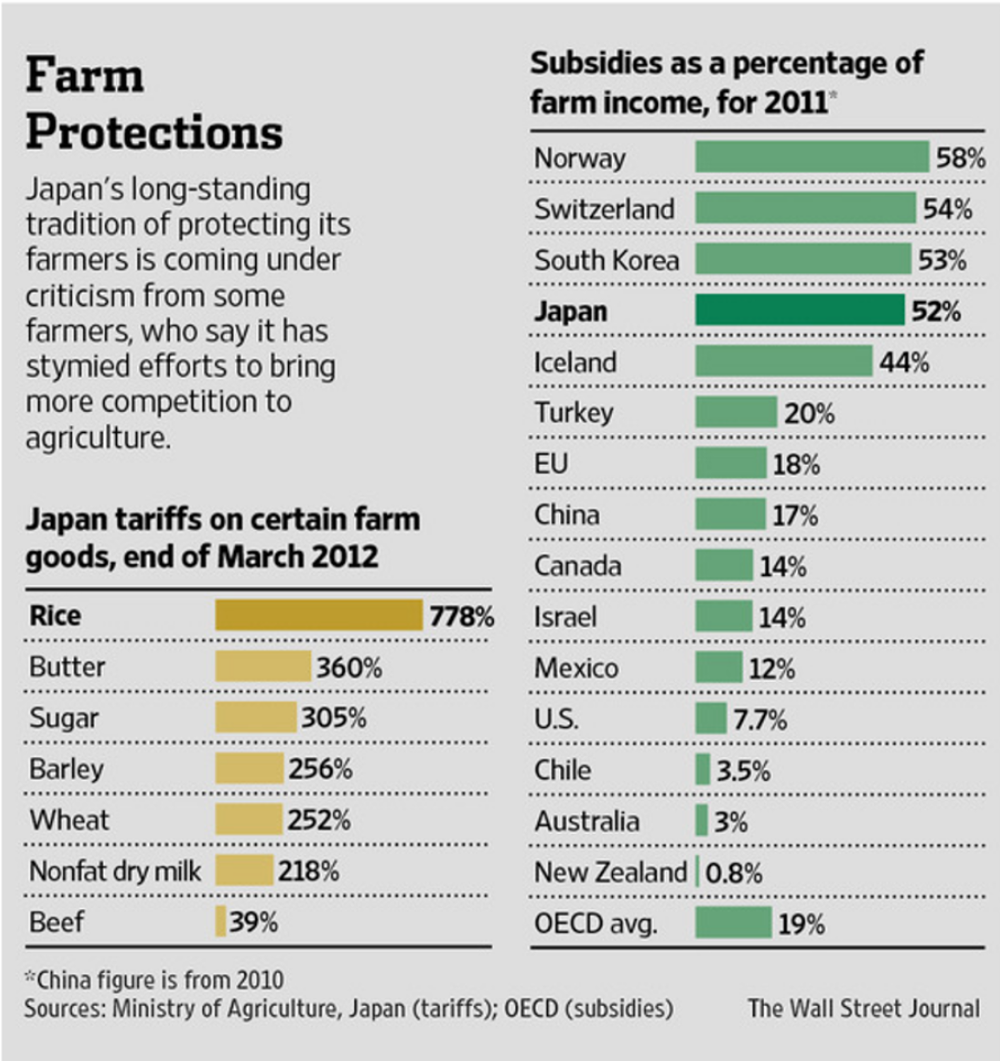
\includegraphics[scale=.8]{jpn_farm_protection}
  \end{figure}
\end{frame}
%--------------------------------------

%--------------------------------------
\begin{frame}
  Consider farm protection in Japan where tariffs allow very little rice to be imported
  \begin{itemize}
    \item Importing 100 EUR worth of rice involves a tariff of 778 EUR 
  \end{itemize}
  \medskip
  Due to land scarcity producing rice in Japan is expensive; country would be better of allowing rice imports.
  However, this would hurt Japanese farmers
  \begin{itemize}
    \item Farmers could move to other industry, such as working in the Toyota factory
    \item Farming skills would probably be useless though    
  \end{itemize}  
  \medskip
  In the short turn farmers can't move to working in another industry.
\end{frame}
%--------------------------------------

%--------------------------------------
\begin{frame}
  Some groups in society oppose free trade due to the potentially negative effect on income
  \begin{itemize}
    \item The specific factors model allows trade to affect income distribution
  \end{itemize}
  \medskip
  The specific factors model assumes that all countries have the same technology, only a different factor mix
  \begin{itemize}
    \item The differences in factor mix leads countries to specialise
    \item e.g. more labour will produce garments, more capital will produce cars
  \end{itemize}
\end{frame}
%--------------------------------------

%--------------------------------------
\begin{frame}
  In the basic model there are 
  \begin{itemize}
  \item Two countries: $Home, Foreign$ 
  \item Two goods: $X,Y$
  \item Three production factors: labour $L$, capital $K$, land $T$
  \end{itemize}
  \medskip
  Two of the three production factors will be sector specific.
\end{frame}
%--------------------------------------

%--------------------------------------
\begin{frame}
Going through the model we will focus on two goods: cloth and food.
Cloth is produced using capital and labour
  \begin{align*}
    Q_c=Q_c(K,L_c)
  \end{align*}
  \medskip
  Food is produced using land and labour
  \begin{align*}
    Q_f=Q_f(T,L_f)
  \end{align*}  
\end{frame}
%--------------------------------------

%--------------------------------------
\begin{frame}
 Similar to the Ricardian model labour $L$ is mobile between the two sectors
  \begin{align*}
    L=L_c+L_f
  \end{align*}
  \medskip
  In addition there are two specific factors capital $K$ and land $T$ which are used in production of only one good.
\end{frame}
%--------------------------------------

%--------------------------------------
\begin{frame}{Cloth production function}
  \begin{figure}
    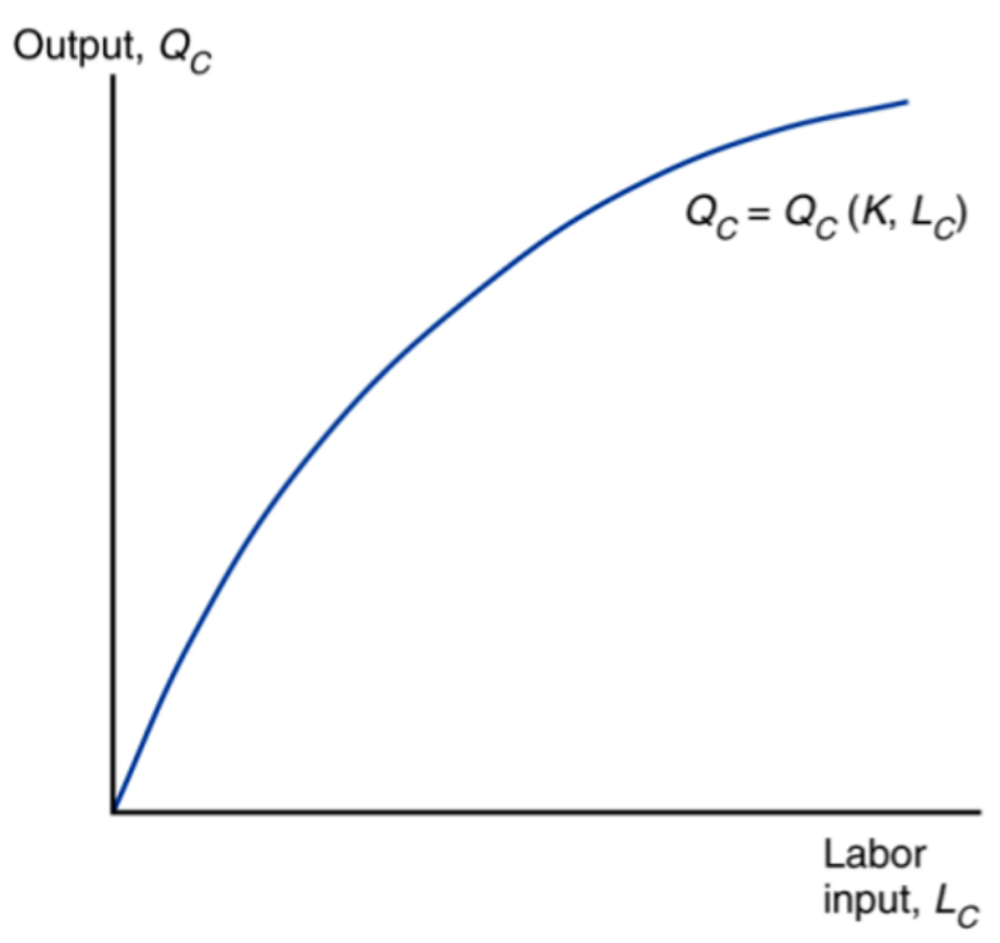
\includegraphics{sf_cloth}
  \end{figure}  
\end{frame}
%--------------------------------------

%--------------------------------------
\begin{frame}
  The specific factors model follows the law of diminishing returns.
  So for example a worker is added to the cloth production process, while the capital level stays constant.
  This means that 
  \begin{itemize}
    \item each worker has less capital to work with
    \item each additional unit of labour adds less output than the last
  \end{itemize}
\end{frame}
%--------------------------------------

%--------------------------------------
\begin{frame}{Labour marginal product}
  \begin{figure}
    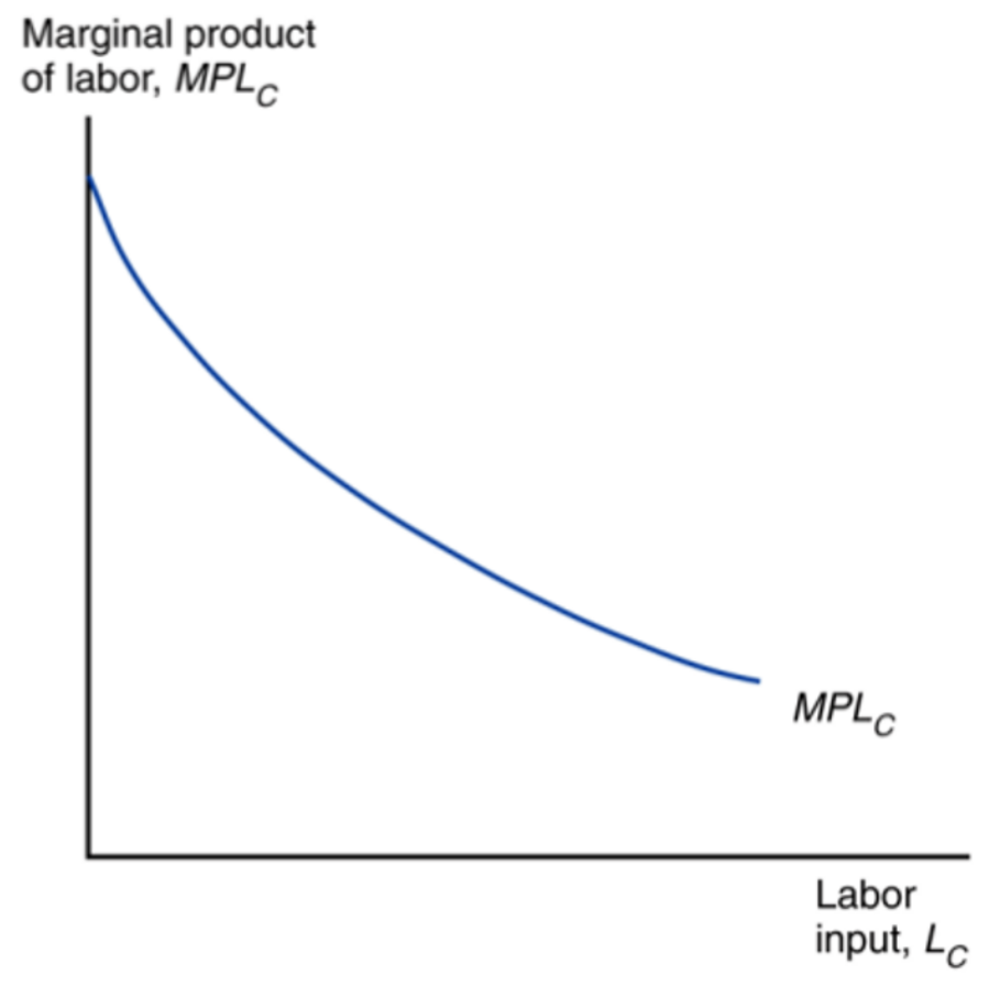
\includegraphics{sf_ml_labour}
  \end{figure}
\end{frame}
%--------------------------------------

%--------------------------------------
\begin{frame}
  To illustrate the PPF we use a four-quadrant diagram
  \begin{enumerate}
    \item Labour allocation shown in lower-left
    \item Cloth production function shown in lower right
    \item Food production function shown in upper left
    \item Combination of food/cloth than can be produces in upper right
  \end{enumerate}
\end{frame}
%--------------------------------------

%--------------------------------------
\begin{frame}{PPF}
  \begin{figure}
    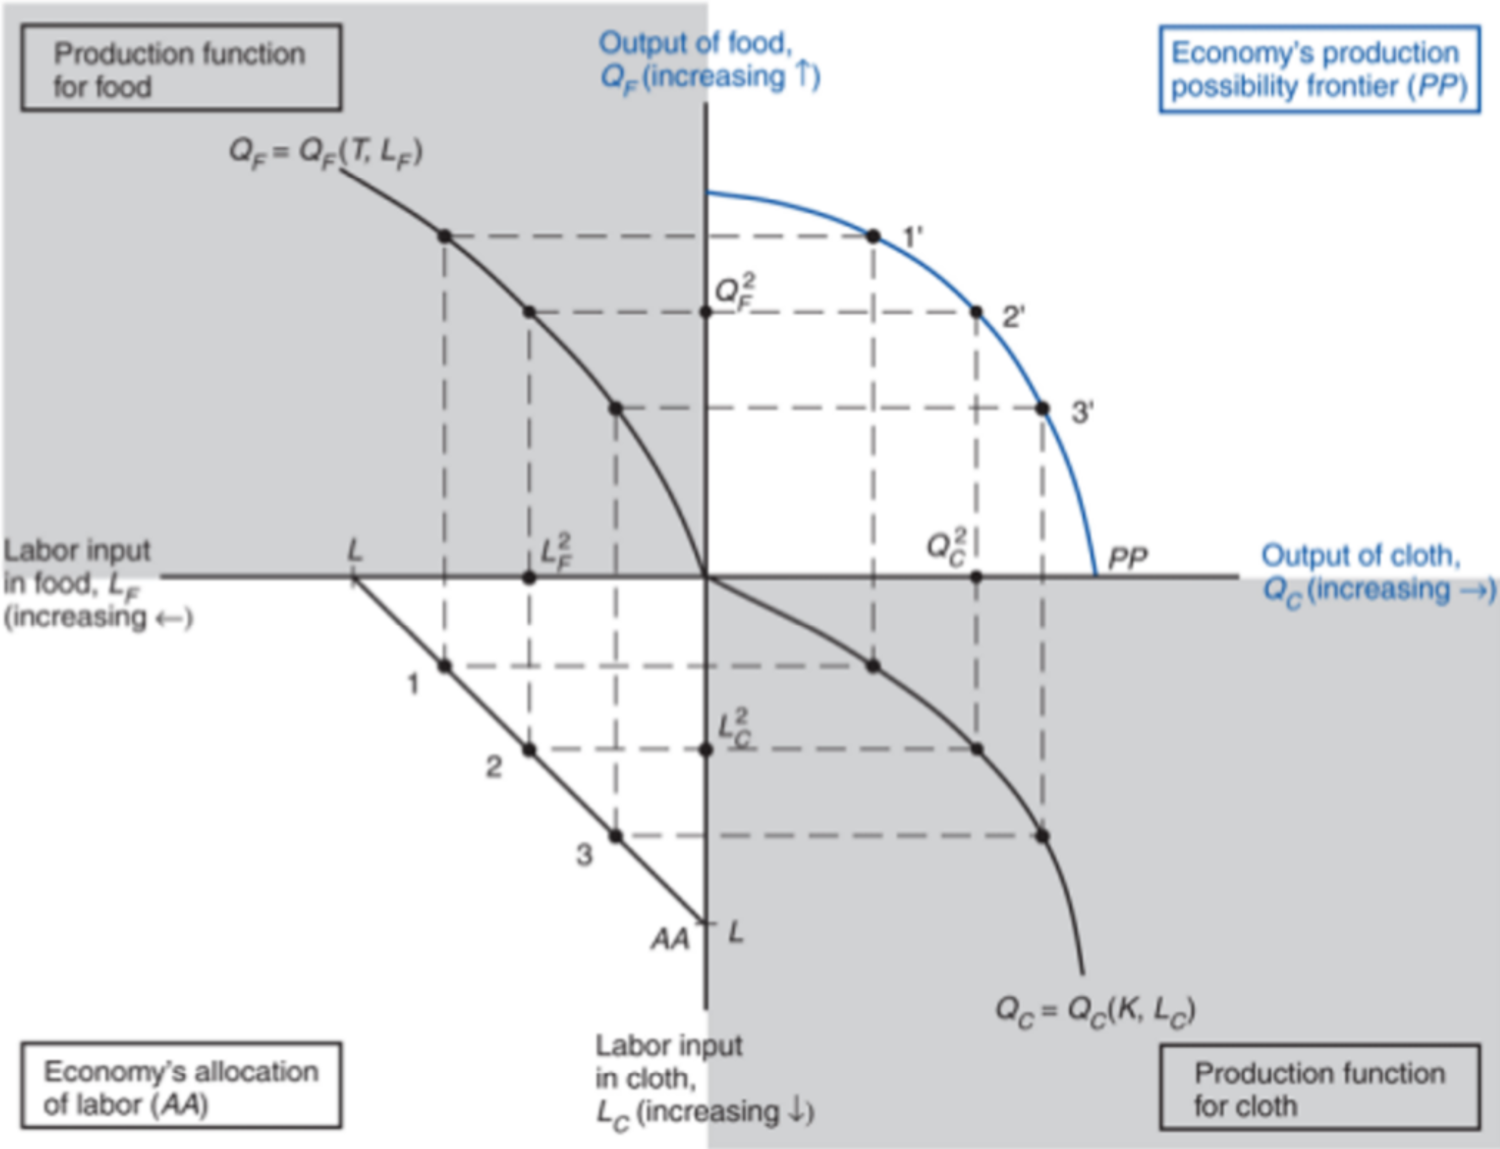
\includegraphics[scale=.8]{sf_ppf}
  \end{figure}
\end{frame}
%--------------------------------------

%--------------------------------------
\begin{frame}
  The Production Possibilities Frontier (PPF) describes the level of output an economy can generate and the slope is given by
  \begin{align*}
    - \frac{Q_L^F(T,L_F)}{Q_L^C(K,L_C)}=-\frac{MPL_F}{MPL_C}
  \end{align*}
  \medskip
  The slope gives the amount of food foregone to produce more clothing.
    \begin{itemize}
      \item Diminishing returns to labour in each sector cause the opportunity costs to rise when an economy produces more of a good
    \end{itemize}
\end{frame}
%--------------------------------------

%--------------------------------------
\begin{frame}
  One important question is which goods will a country produce after it opens up to trade?
  The specific factors model builds on the idea of comparative advantage of Ricardo
  \begin{itemize}
    \item Each country will export the good in which it has a comparative advantage
  \end{itemize}
  \medskip
  The comparative advantage will be determined by the specific factor in which it is relatively abundant. 
    \begin{itemize}
    \item e.g. a capital intensive good (cloth) will be produced by the capital abundant country; food will be produced by the land abundant country    
  \end{itemize}
  \medskip  
  Importantly there will be incomplete specialisation. 
  \begin{itemize}
    \item The country will produce on that point of the PPF where the slope equals the relative price of the two goods
  \end{itemize}
\end{frame}
%--------------------------------------

%--------------------------------------
\begin{frame}
  The specific factors model accounts for the effect of trade on income. 
  Let's have a look at the determination of wages and prices. 
  For each sector wage $w$ will equal the marginal product of labour $MPL$ times the price $p$ or  
    \begin{align*}
    w = p_c\cdot MPL_c = p_f \cdot MPL_F     
  \end{align*}
  \medskip
  Note that due to labour mobility both sectors will pay the same wage.
  In terms of relative prices we have
  \begin{align*}
    - \frac{p_c}{p_f}=-\frac{MPL_F}{MPL_C}
  \end{align*}  
\end{frame}
%--------------------------------------

%--------------------------------------
\begin{frame}{Labour allocation in autarky}
  \begin{figure}
    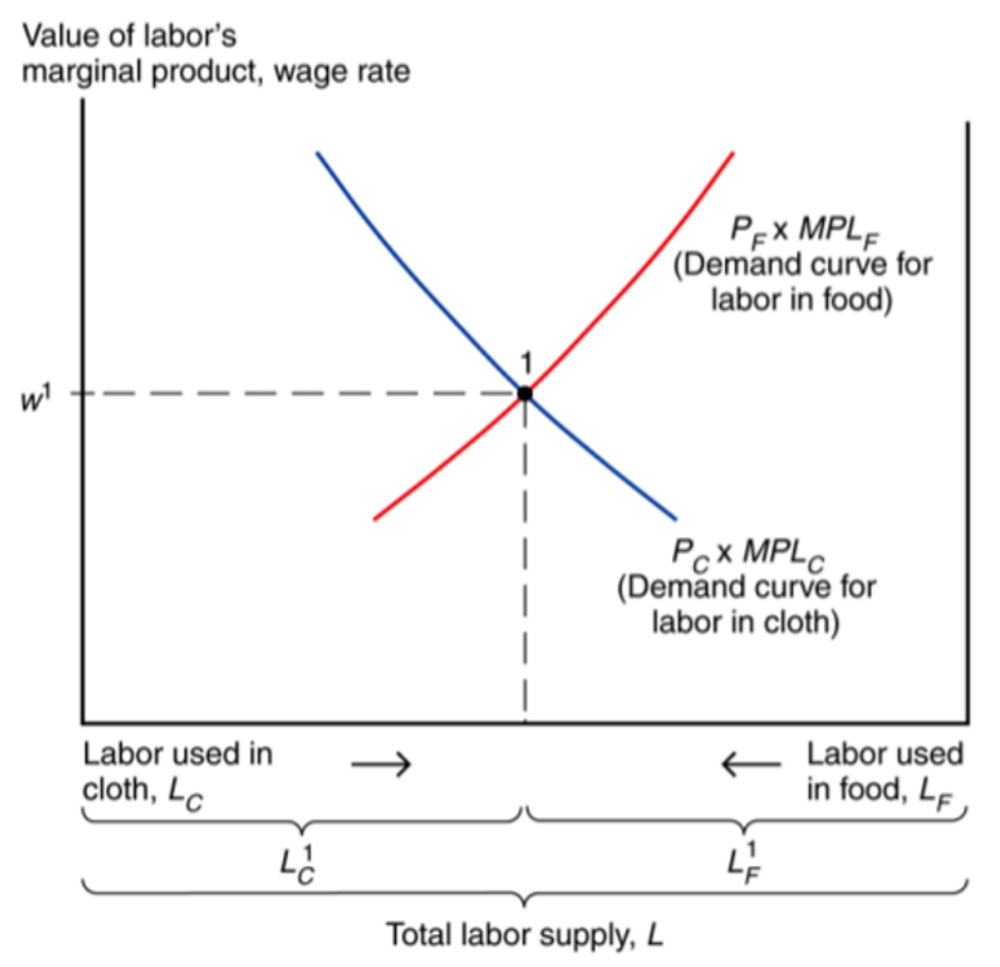
\includegraphics{sf_s_labour}
  \end{figure}
\end{frame}
%--------------------------------------

%--------------------------------------
\begin{frame}{Production function}
  \begin{figure}
    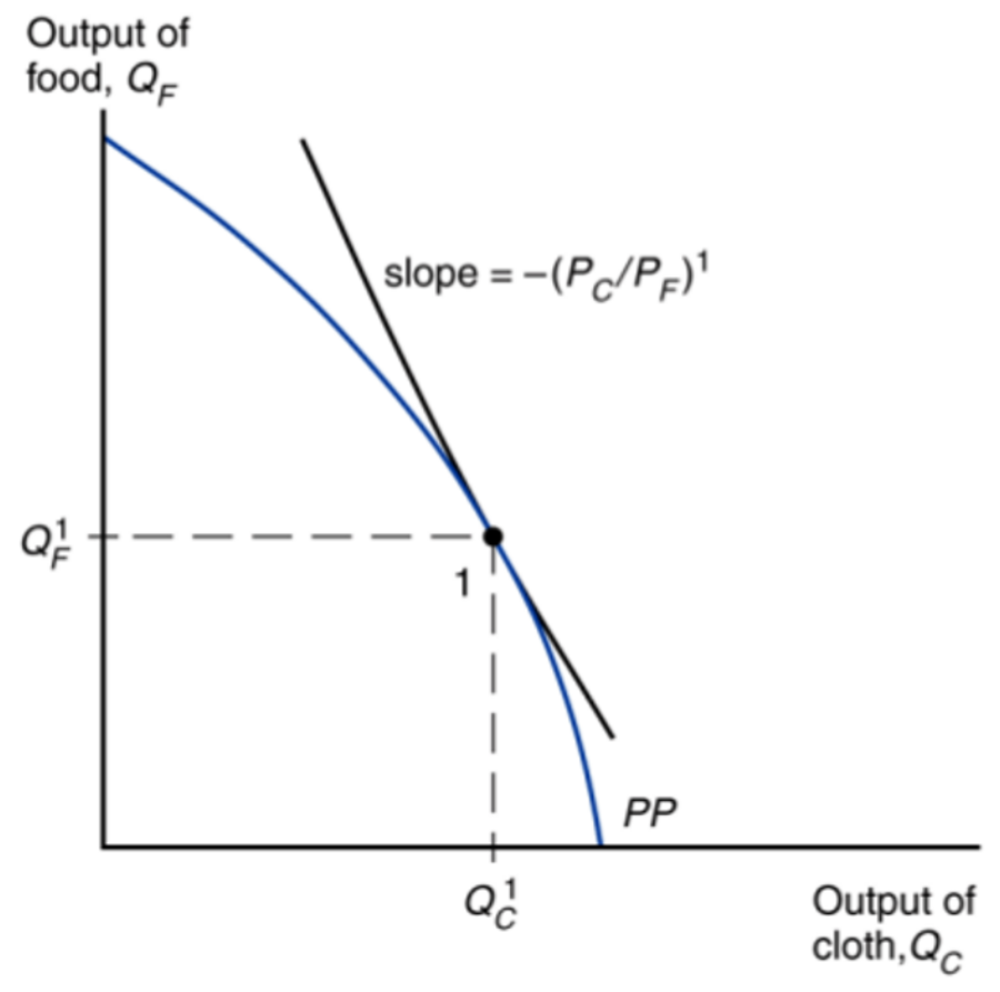
\includegraphics{sf_pf}
  \end{figure}    
\end{frame}
%--------------------------------------

%--------------------------------------
\begin{frame}
  Besides labour we also have capital and land as production factors, and the returns to these are given by
  \begin{align*}
    r_K = \frac{p_c \cdot Q_c -w \cdot L_c}{K}\\
    r_T = \frac{p_f \cdot Q_f - w \cdot L_f}{T}
  \end{align*}
  \begin{itemize}
    \item $K, T$ earn what is left from sales revenues $pQ$ after labour is paid $wL$
  \end{itemize}
\end{frame}
%--------------------------------------

%--------------------------------------
\begin{frame}
  We can now check what will happen to labour allocation and the income distribution following a change in prices.
  Here we will consider a change in 
  \begin{enumerate}
    \item Prices in equal proportions
    \item Relative prices
  \end{enumerate}
\end{frame}
%--------------------------------------

%--------------------------------------
\begin{frame}{Equal proportional change in prices}
  \begin{figure}
    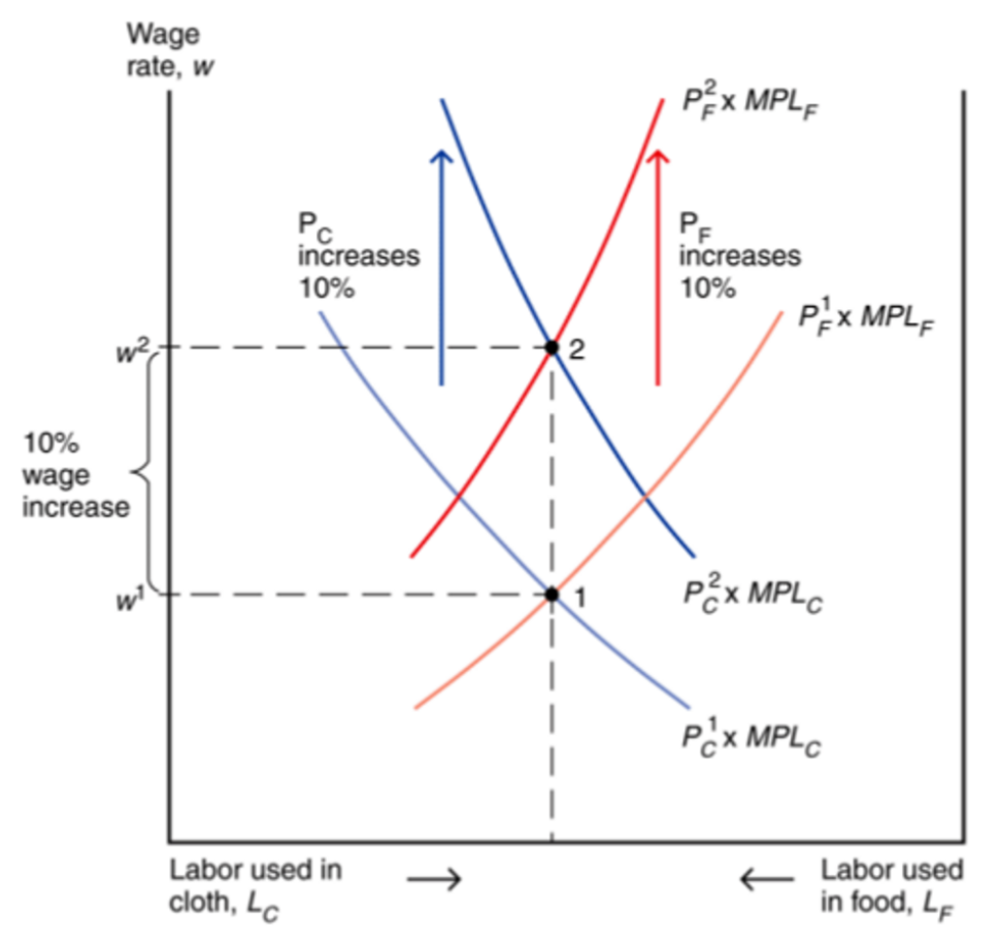
\includegraphics{sf_wages}
  \end{figure}
\end{frame}
%--------------------------------------

%--------------------------------------
\begin{frame}
  Following an equal proportional change in price no real changes occur
  \begin{itemize}
    \item $w$ rises in the same proportion, real wages are unaffected
    \item Real incomes of capital and landowners stay the same
  \end{itemize}
\end{frame}
%--------------------------------------

%--------------------------------------
\begin{frame}{Increase in the price of cloth}
  \begin{figure}
    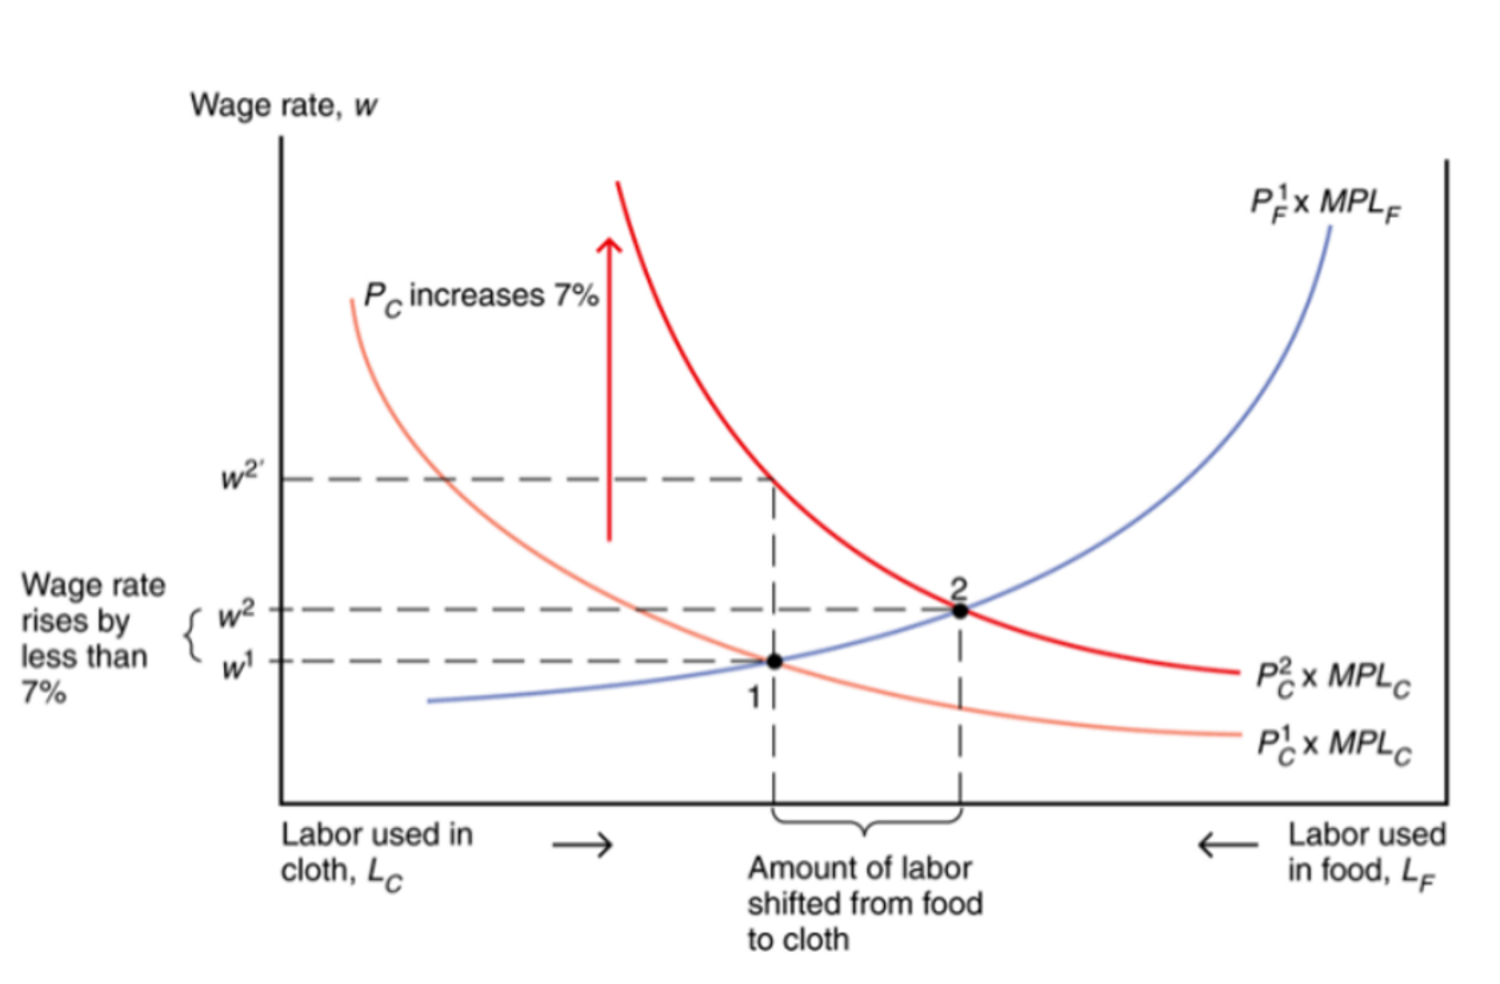
\includegraphics[scale=.9]{sf_price_increase}
  \end{figure}
\end{frame}
%--------------------------------------

%--------------------------------------
\begin{frame}
  Following a change in relative prices, when $p$ changes in one sector does lead to changes
  \begin{enumerate}
    \item Labour moves to sector with higher prices
    \item Output in other sector decreases
  \end{enumerate}
  $w$ does not increase as much as $p$ given that the marginal product of labour will decrease
\end{frame}
%--------------------------------------

%--------------------------------------
\begin{frame}{Effect of cloth price change on output}
  \begin{figure}
    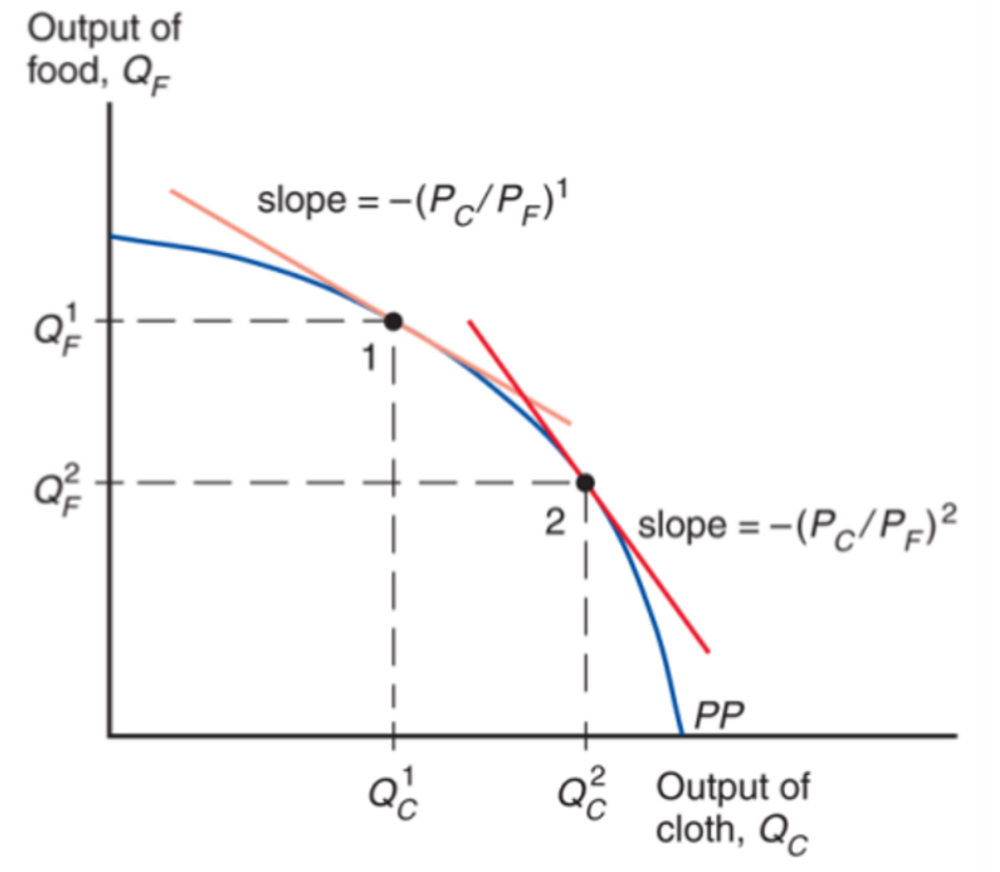
\includegraphics{sf_output}
  \end{figure}
\end{frame}
%--------------------------------------

%--------------------------------------
\begin{frame}
  The relative price change also affects real income
  \begin{enumerate}
    \item Capital owners are better of due to positive price shock in capital intensive sector
    \begin{itemize}
      \item $r_k$ increases, marginal product of $K$ is expected to increase
    \end{itemize}
    \medskip
    \item Landowners are worse off since land is not a production factor in the cloth industry
    \begin{itemize}
      \item $r_t$ decreases, marginal product of $T$ is expected to decrease
    \end{itemize}
    \medskip
    \item Effect of workers is ambiguous; depends on relative importance of cloth and food in consumption
    \begin{itemize}
      \item Wages increase, but so does the textile price
      \item Can afford more food but less clothes
    \end{itemize}
  \end{enumerate}
\end{frame}
%--------------------------------------

%--------------------------------------
\begin{frame}{Income distribution in cloth sector}
  \begin{figure}
    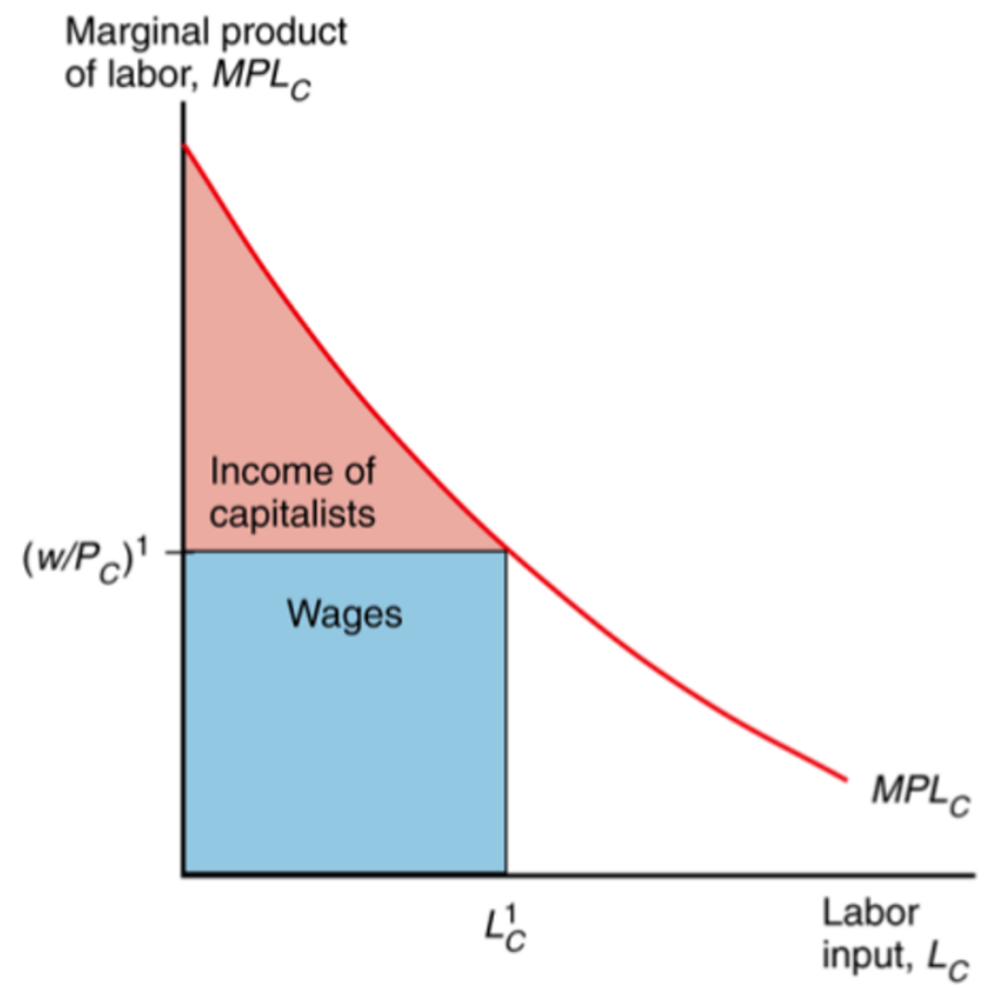
\includegraphics[scale=.9]{sf_income1}
  \end{figure}
\end{frame}
%--------------------------------------

%--------------------------------------
\begin{frame}{Effect of price change on income capital owners}
  \begin{figure}
    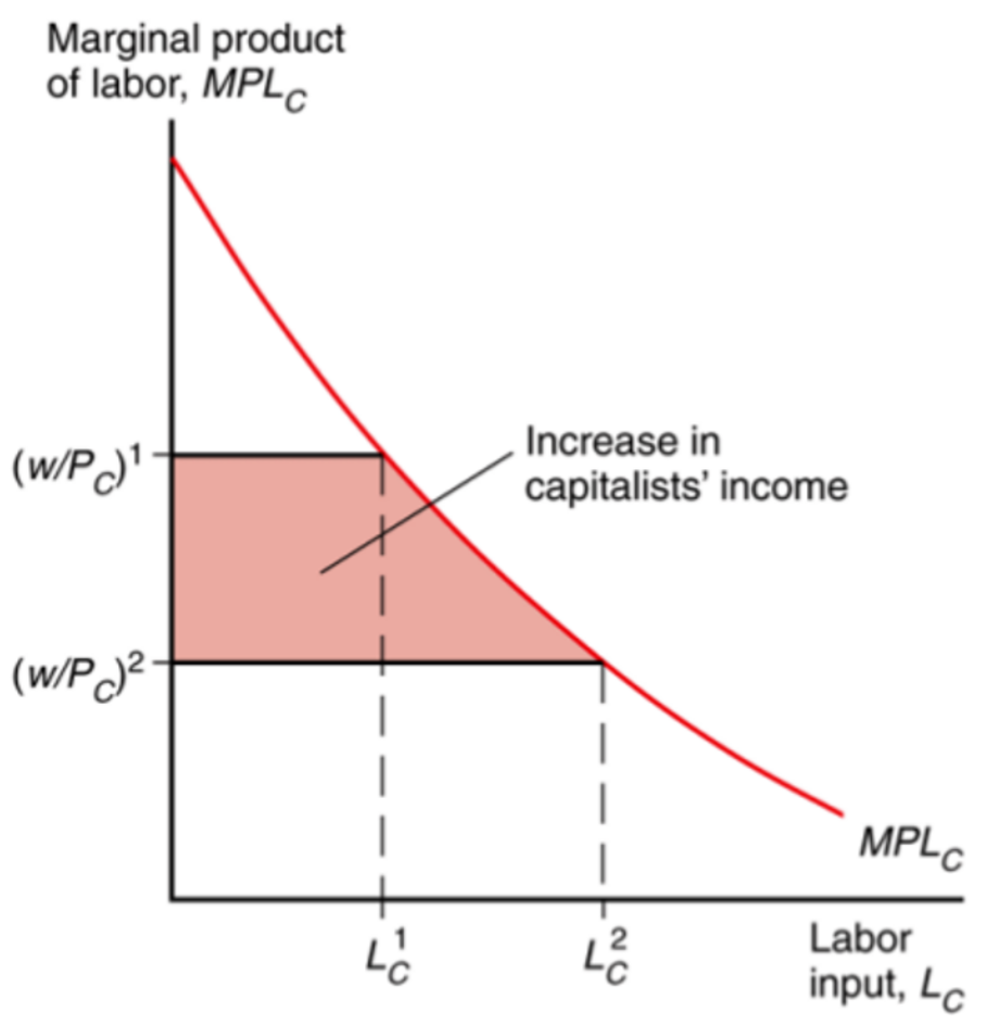
\includegraphics[scale=.9]{sf_income2}
  \end{figure}
\end{frame}
%--------------------------------------

%--------------------------------------
\begin{frame}{Effect of price change on income landowners}
  \begin{figure}
    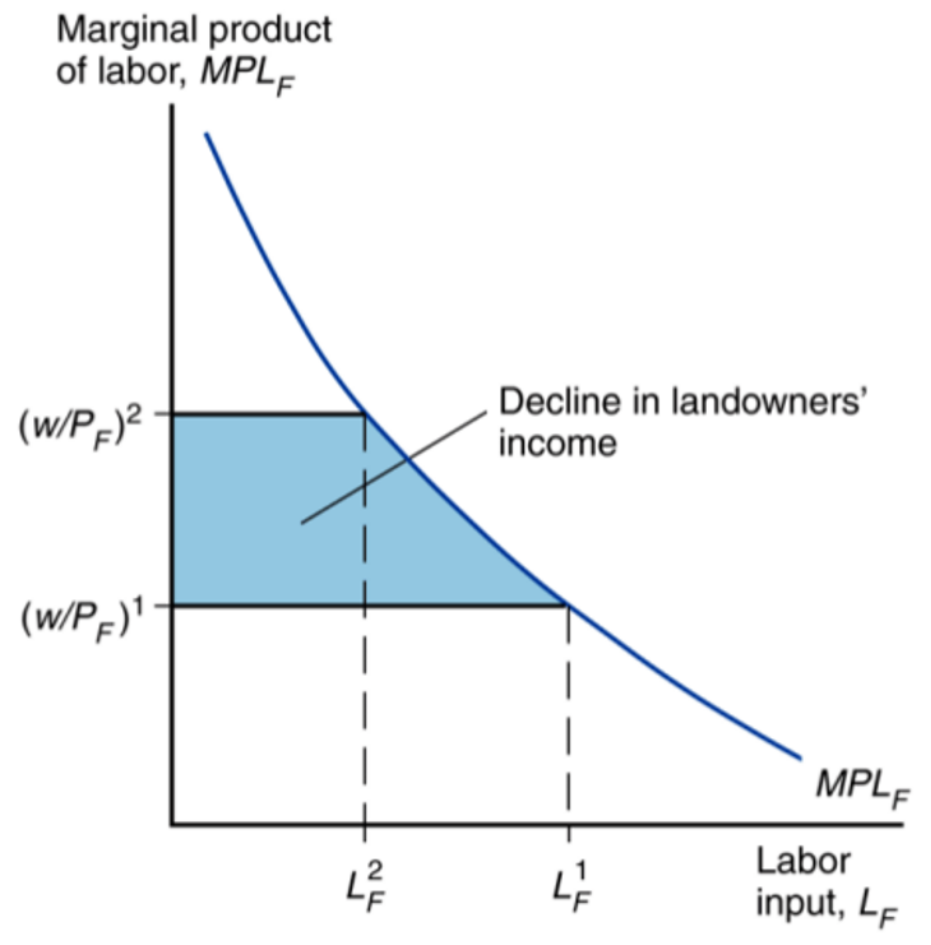
\includegraphics{sf_income3}
  \end{figure}
\end{frame}
%--------------------------------------

%--------------------------------------
\begin{frame}
 Note the political implications of the model: the issue of free trade will diametrically oppose the two specific factors each one vying for the support of the mobile factor.
\end{frame}
%--------------------------------------

%--------------------------------------
\begin{frame}
  Opening up to trade is the same as a change in relative prices which means that some will gain and others will lose. 
  The direction of the change depends on two factors:
  \begin{enumerate}
    \item Economy's relative demand and supply
    \item World's relative demand and supply
  \end{enumerate}
  \medskip
  In an economy whose relative supply of cloth is larger than for the world as a whole, opening up to trade will increase the relative price of cloth. 
\end{frame}
%--------------------------------------

%--------------------------------------
\begin{frame}{Relative prices under international trade}
  \begin{figure}
    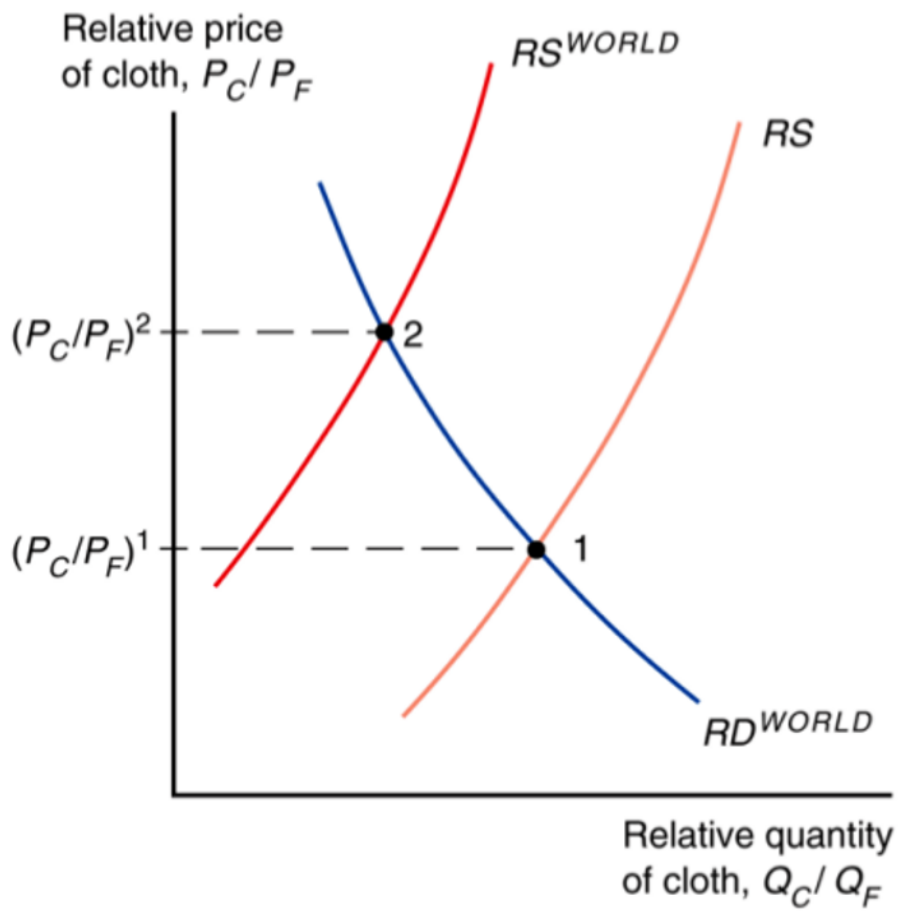
\includegraphics{sf_rprices}
  \end{figure}
\end{frame}
%--------------------------------------


%--------------------------------------
\begin{frame}
 In the model relative prices will converge due to international trade.
 Let's consider two trading economies
 \begin{enumerate}
    \item Japan
    \item USA
  \end{enumerate} 
  \medskip
  Assume that they have the same relative demand, which entails that relative supply is the source of international trade. 
  Relative supply might differ because the countries are different in terms of
 \begin{itemize}
   \item Technology level
   \item Factors of production
 \end{itemize} 
\end{frame}
%--------------------------------------

%--------------------------------------
\begin{frame}
  Also assume that both countries produce the same two goods
  \begin{enumerate}
    \item Manufactures, which are capital intensive
    \item Food, which is land intensive
  \end{enumerate}
  \medskip
  While Japan has more capital per worker, the USA will have more land. 
   \begin{itemize}
   \item This means that the autarky relative price in Japan of a capital intensive good is lower compared to that of the USA
 \end{itemize}
\end{frame}
%-------------------------------------- 

%--------------------------------------
\begin{frame}
  \begin{figure}
    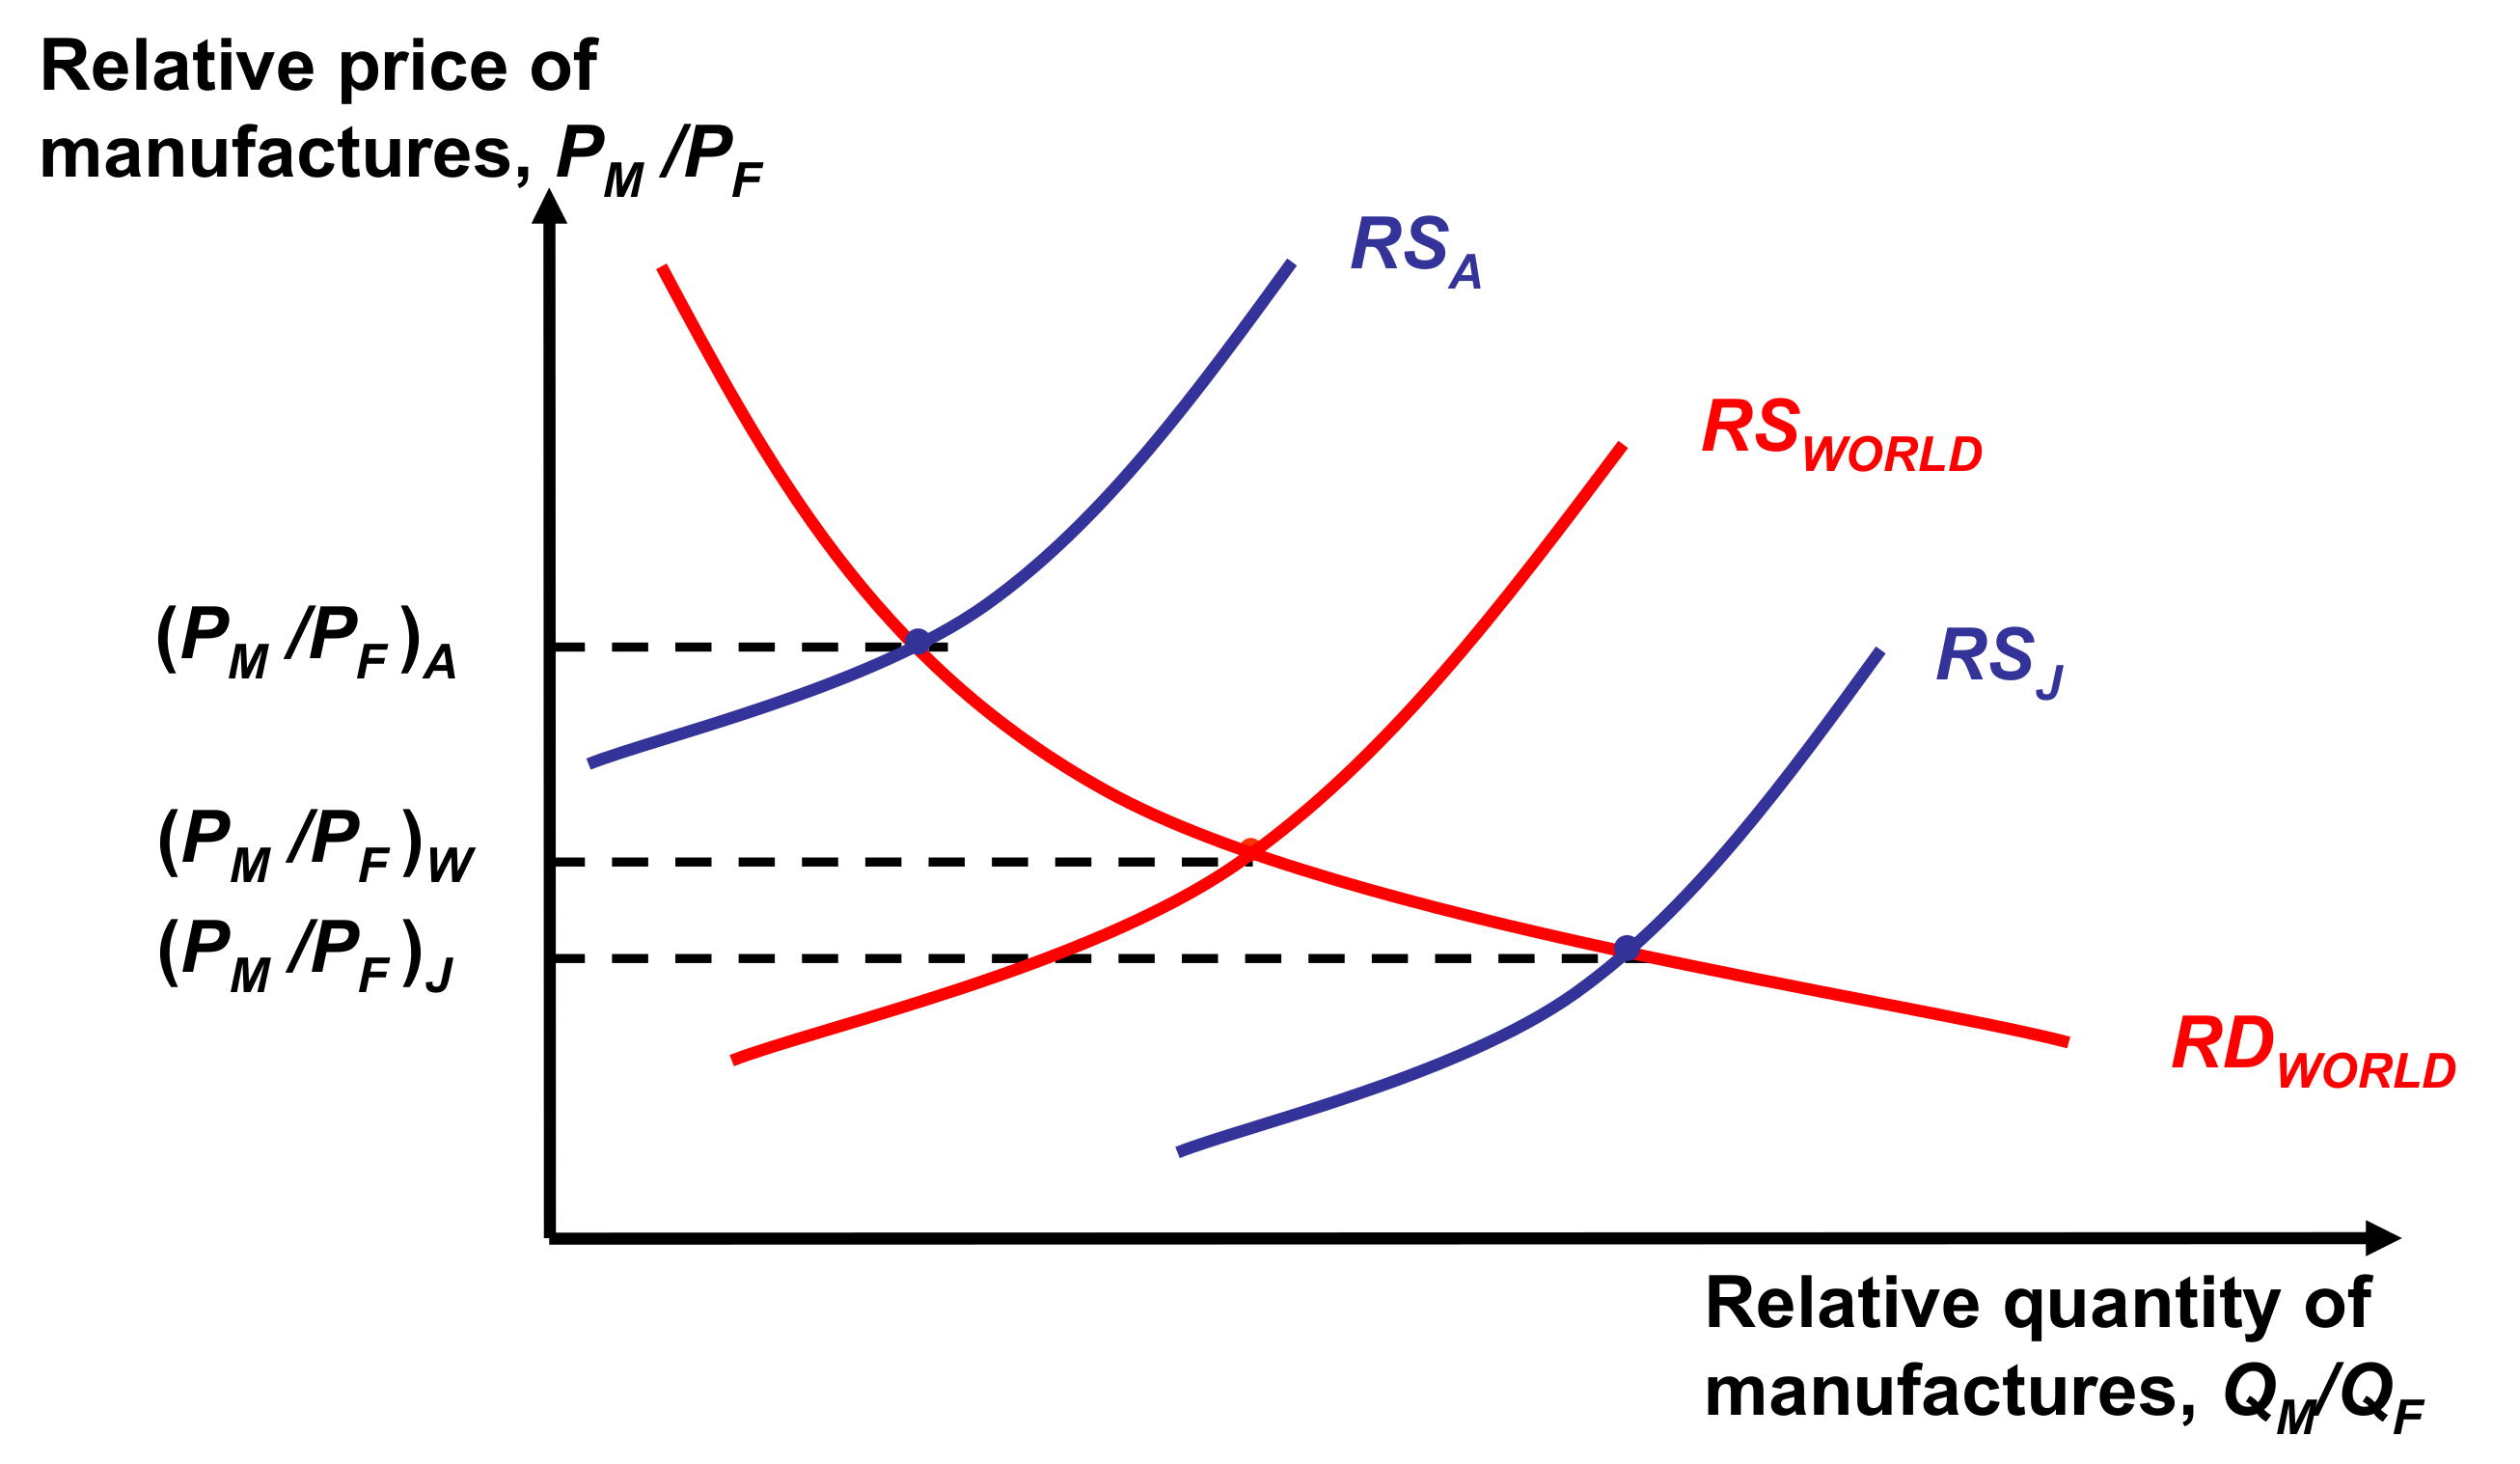
\includegraphics[scale=.5]{usa_jpn.png}
  \end{figure}
\end{frame}
%--------------------------------------

%--------------------------------------
\begin{frame}
  The model predicts that the economy as a whole will gain: 
  In autarky a country's output must equal its consumption whereas trade allows the consumption mix to differ from production mix.\\
  Consumption is constrained by
  \begin{align*}
    p_c \cdot D_c + p_f \cdot D_f = p_c \cdot Q_c + p_f \cdot Q_f
  \end{align*}
  \medskip
  i.e. a country cannot spend more than it earns.  
\end{frame}
%--------------------------------------

%--------------------------------------
\begin{frame}
 Under free trade it is able to afford amounts of cloth and food that it is not able to produce itself
  \begin{align*}
    D_f - Q_f = \frac{p_c}{p_f} \cdot (Q_c-D_c)
  \end{align*}
  \medskip
  i.e. it imports food equal to the relative price of cloth times cloth exported.
\end{frame}
%--------------------------------------

%--------------------------------------
\begin{frame}
  When a country opens up to trade the factor prices will change
  \begin{itemize}
    \item Trade benefits factor that is specific to the export sector
    \item Trade hurts factor that is specific to the import-competing sector
    \item Effect on mobile factor is ambiguous
  \end{itemize}
  \medskip
  Trade will expand consumption possibilities but also creates winners and losers
  \begin{itemize}
    \item Losers can be compensated by income redistribution
  \end{itemize}  
\end{frame}
%--------------------------------------

%--------------------------------------
\begin{frame}
Opening up to trade there will also be a shift in employment from the import-competing to the export sector.
\medskip
  \begin{itemize}
    \item Process not instantaneous: some will be unemployed
    \item No strong correlation between unemployment and trade though
  \end{itemize}
\end{frame}
%--------------------------------------

%--------------------------------------
\begin{frame}{Unemployment and import penetration in Spain}
  \begin{figure}
    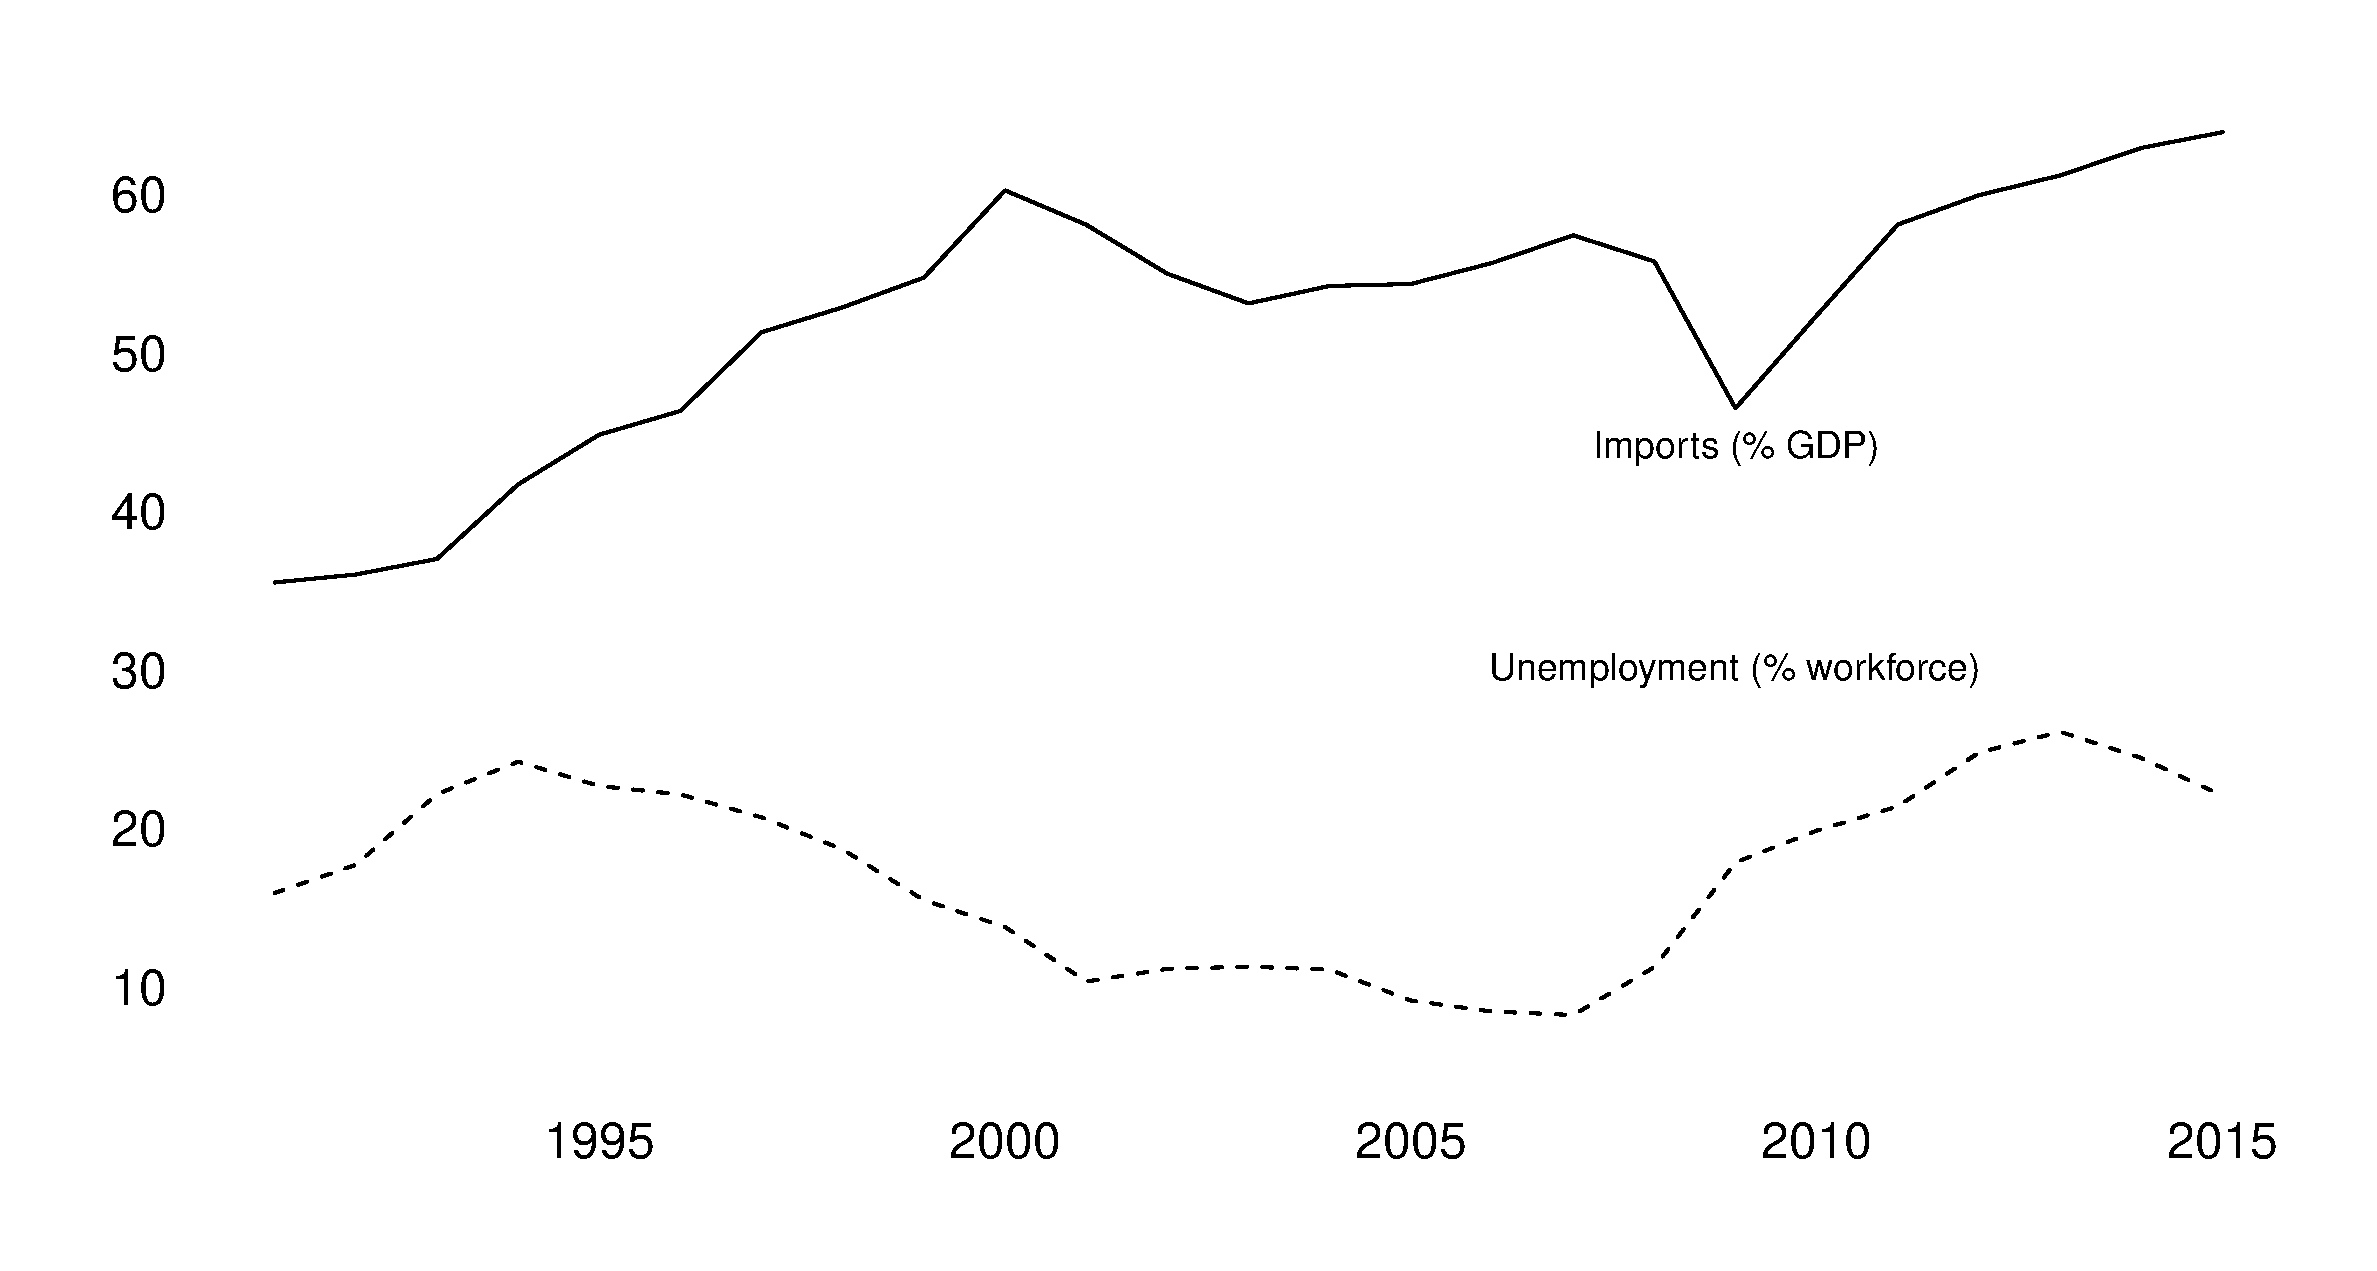
\includegraphics[scale=.3]{import}
  \end{figure}
\end{frame}
%--------------------------------------

%--------------------------------------
\begin{frame}
 Besides import-competing sectors, trade can also hurt some exporting sectors following a windfall in one particular sector.
 \begin{itemize}
  \item The dynamics are similar to a change in relative prices
 \end{itemize}
 \medskip
 This is known as the Dutch disease.
\end{frame}
%--------------------------------------


%--------------------------------------
\begin{frame}
  \begin{figure}
    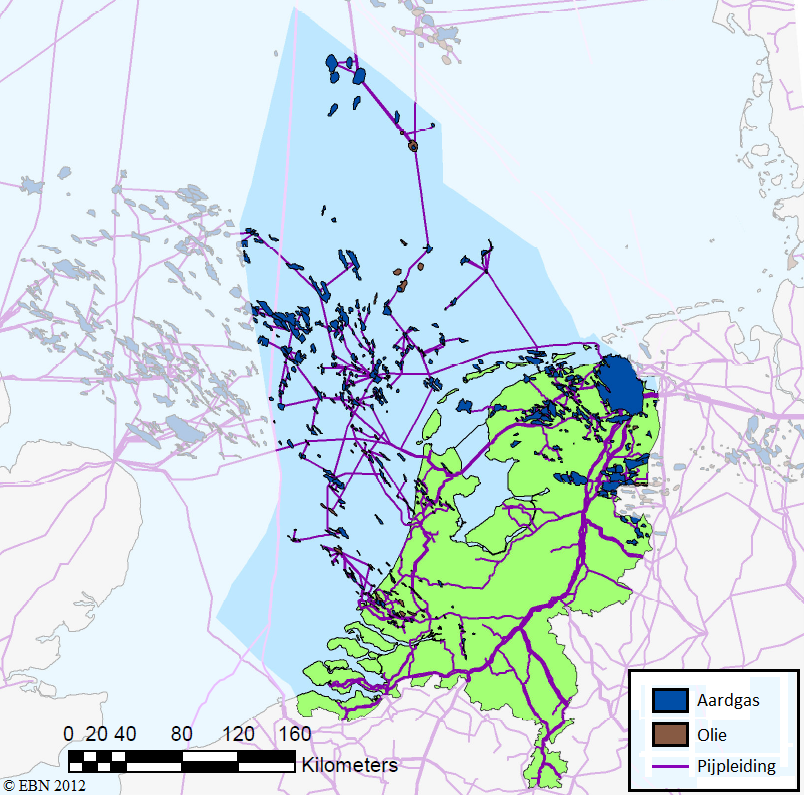
\includegraphics[scale=.4]{aardgas.png}
  \end{figure}
\end{frame}
%--------------------------------------

%--------------------------------------
\begin{frame}
 In 1959 the Dutch Petroleum Company found the largest natural gas field in Europe near Slochteren in the province of Groningen
 \begin{itemize}
   \item Besides the gas field in Groningen there are about 250 other fields on land and in the North Sea
 \end{itemize}
 \medskip
 After creating a domestic gas market the Dutch became the 9th largest exporter of natural gas in the world and the largest in Europe
 \begin{itemize}
  \item Currently the Netherlands rank 17th due to a decrease in production.
 \end{itemize}
\end{frame}
%--------------------------------------

%--------------------------------------
\begin{frame}
  \begin{figure}
    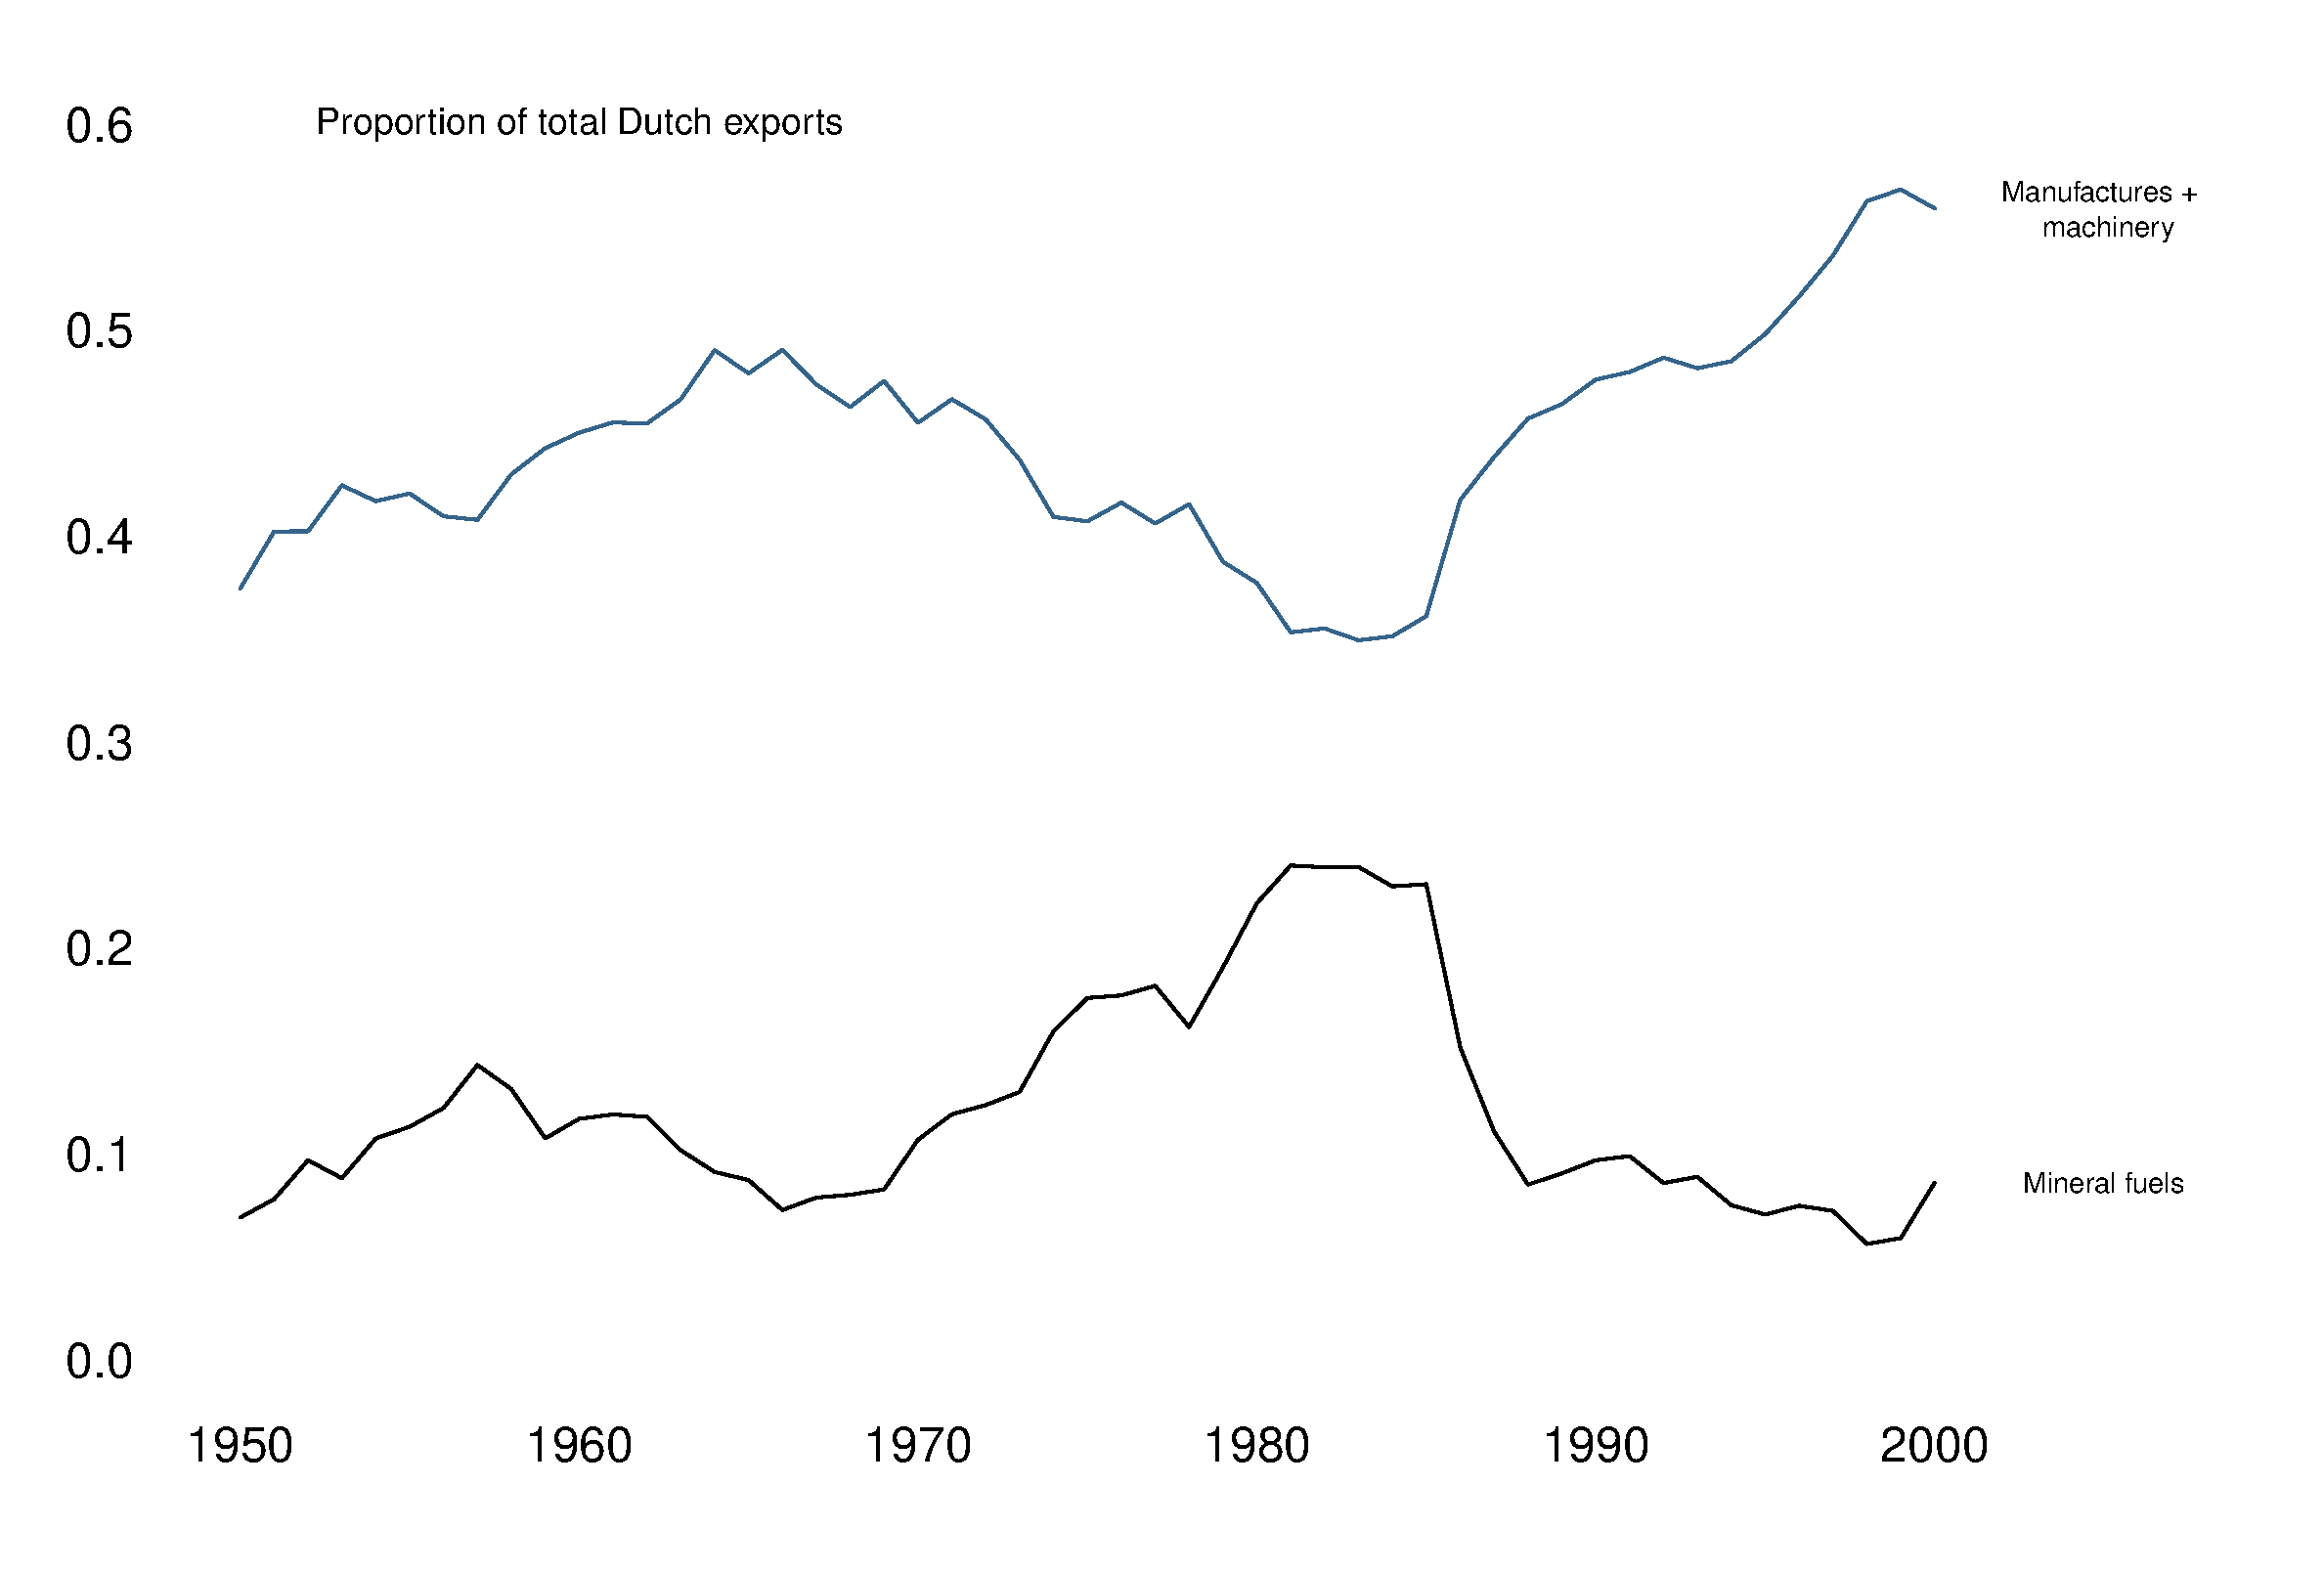
\includegraphics[scale=.3]{dutch_exports.eps}
  \end{figure}
\end{frame}
%--------------------------------------

%--------------------------------------
\begin{frame}
 The expansion of the gas sector made other sectors such as manufacturing less competitive.
 \begin{itemize}
   \item The manufacturing sector contracted becoming "too" small.
 \end{itemize}
 \medskip
 Why is this a problem?
 \begin{itemize}
   \item A trading sector will benefit most from learning-by-doing
   \item Shrinking the sector will reduce learning-by-doing and reduce growth
 \end{itemize}
 \medskip
 In the case of the Netherlands the natural resource revenues made the national currency appreciate in value, making it harder for other sectors to export.
 \end{frame}
%--------------------------------------

%--------------------------------------
\begin{frame}
  More broadly in terms of international trade we can define the \textbf{Dutch disease} as
  \begin{quote}
  A favourable change in the economic development of one exporting sector that has adverse consequences for other exporting sectors.
  \end{quote}
\end{frame}
%--------------------------------------

%--------------------------------------
\begin{frame}
 More general: Suppose that there are $N$ industries which produce and sell their products on the world market
  \begin{itemize}
    \item They each need labour $L$ for their production, combined with another factor 
    \item Recall that $L$ is mobile across industries
  \end{itemize}
  \medskip
  When the world market price for one industry $i$ increases, this industry will expand leading to an increase in wage $w$.\footnote{Capital will also be drawn towards the industry experiencing the windfall.}
  This wage increase will hamper the other $N-i$ exporting industries
  \begin{itemize}
    \item They face higher marginal costs due to a wage increase
    \item Yet the world market price for their product remained the same 
  \end{itemize}
\end{frame}
%--------------------------------------


%--------------------------------------
\begin{frame}
 \begin{figure}
   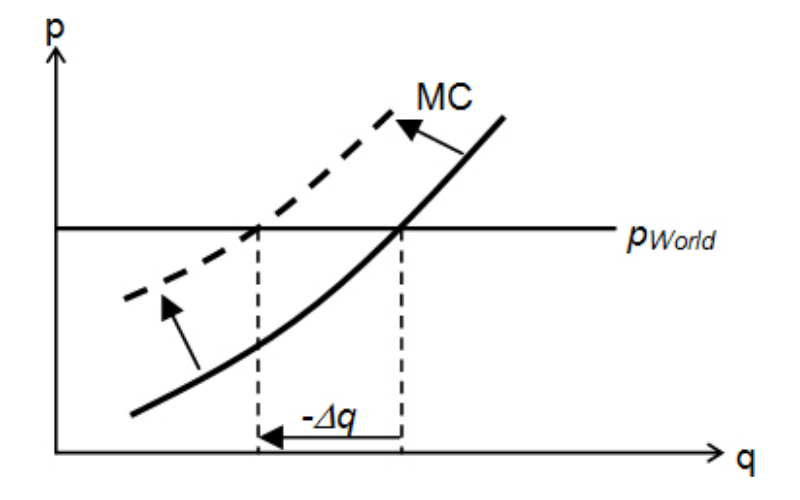
\includegraphics[scale=1.2]{dutch_disease.png}
 \end{figure}
\end{frame}
%--------------------------------------

%--------------------------------------
\begin{frame}
  We can also consider the movement of production factors across countries rather than only industries, such as   
  \begin{itemize}
    \item Labour migration
    \item International borrowing and lending
    \item FDI
  \end{itemize}
  \medskip
  Movement of production factors can be politically sensitive and subject to restrictions.
\end{frame}
%--------------------------------------

%--------------------------------------
\begin{frame}
Let's focus on labour mobility. 
Suppose that there are two countries, $Home,Foreign$, who produce one non-traded good using two production factors
  \begin{enumerate}
    \item Land, which is fixed
    \item Labour, which can move across countries and workers will migrate to the country with the higher wage
  \end{enumerate}
  \medskip 
  Let's assume that wages in $Home$ are lower than in $Foreign$ due to lower productivity.
  \begin{itemize}
    \item This means that $Home$ workers want to migrate to $Foreign$ 
  \end{itemize}  
  \medskip
  Without obstacles workers will migrate until purchasing power of wages is equal across countries.\footnote{In real life this doesn't happen due to barriers to migration.}  
\end{frame}
%--------------------------------------

%--------------------------------------
\begin{frame}{Labour mobility across countries}
  \begin{figure}
    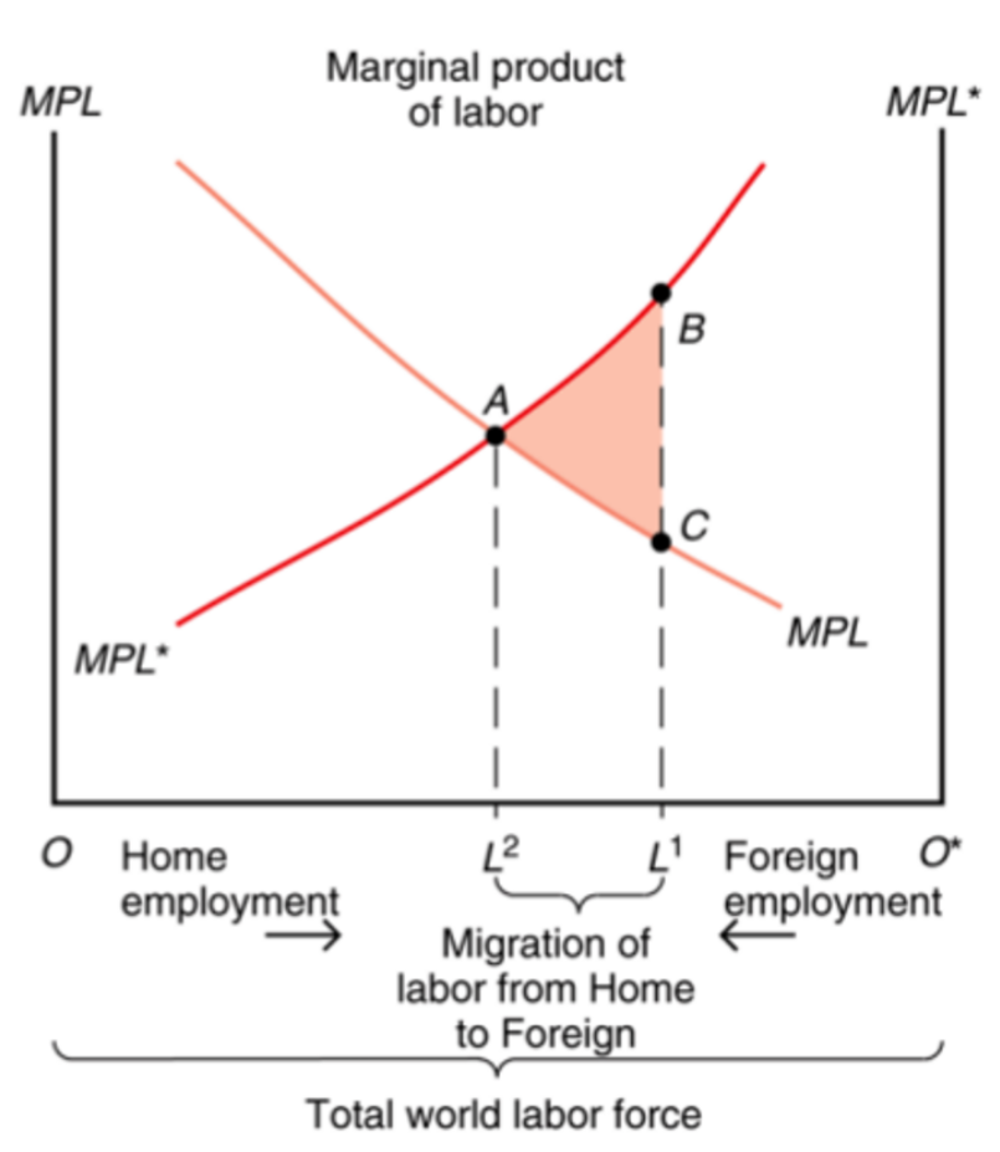
\includegraphics[scale=.8]{sf_lmobility}
  \end{figure}
\end{frame}
%--------------------------------------

%--------------------------------------
\begin{frame}
  In this example workers in $Home$ will benefit while those in $Foreign$ will be hurt.
  What is the effect on owners of the other production factor, land?
  \begin{enumerate}
    \item $Foreign$ landowners will benefit by labour inflow; decreasing real wages and increasing output
    \item $Home$ landowners will be hurt by labour outflow; increasing real wages and decreasing output
  \end{enumerate}
  \medskip
  From an economic perspective there is a case for barrier-free migration as it increases world output as $L$ moves to more productive areas.
  \begin{itemize}
    \item The value of world output is maximised when marginal productivity of labour is equal across countries     
  \end{itemize}
\end{frame}
%--------------------------------------

%--------------------------------------
\begin{frame}{Real wages in origin and destination countries}
\framesubtitle{source: Williamson, 1995}
\begin{table}
\scalebox{.7}{
  \begin{tabular}{lcc}
  ~   & Real wage 1870, US = 100 & Increase real wage 1870-1913 (\%)\\
      \hline \\[-1.8ex]\\	
      \textit{Origin countries} & ~   &~\\
      Ireland     & 43  & 84\\
      Italy       & 23  & 112\\
      Norway      & 24  & 193\\
      Sweden      & 24  & 250\\    
      \\[-1.8ex]\\
      \textit{Destination countries}  & ~ & ~\\
      Argentina   & 53  & 51\\
      Australia   & 110 & 1\\
      Canada      & 86  & 121\\
      US          & 100 & 47\\      
  \end{tabular}}
\end{table}  
\end{frame}
%--------------------------------------

%--------------------------------------
\begin{frame}
 \textbf{Food for thought:}\\
 By 1910 about 14 million immigrants were living in the USA on a population of 92 million.
 Who do you think would have favoured migration in the USA?
 \begin{enumerate}
   \item Capitalists
   \item Landowners
   \item Labour unions
 \end{enumerate}
\end{frame}
%--------------------------------------

%--------------------------------------
\begin{frame}{Recall: Migration flows between 2005-2010}
  \begin{figure}
    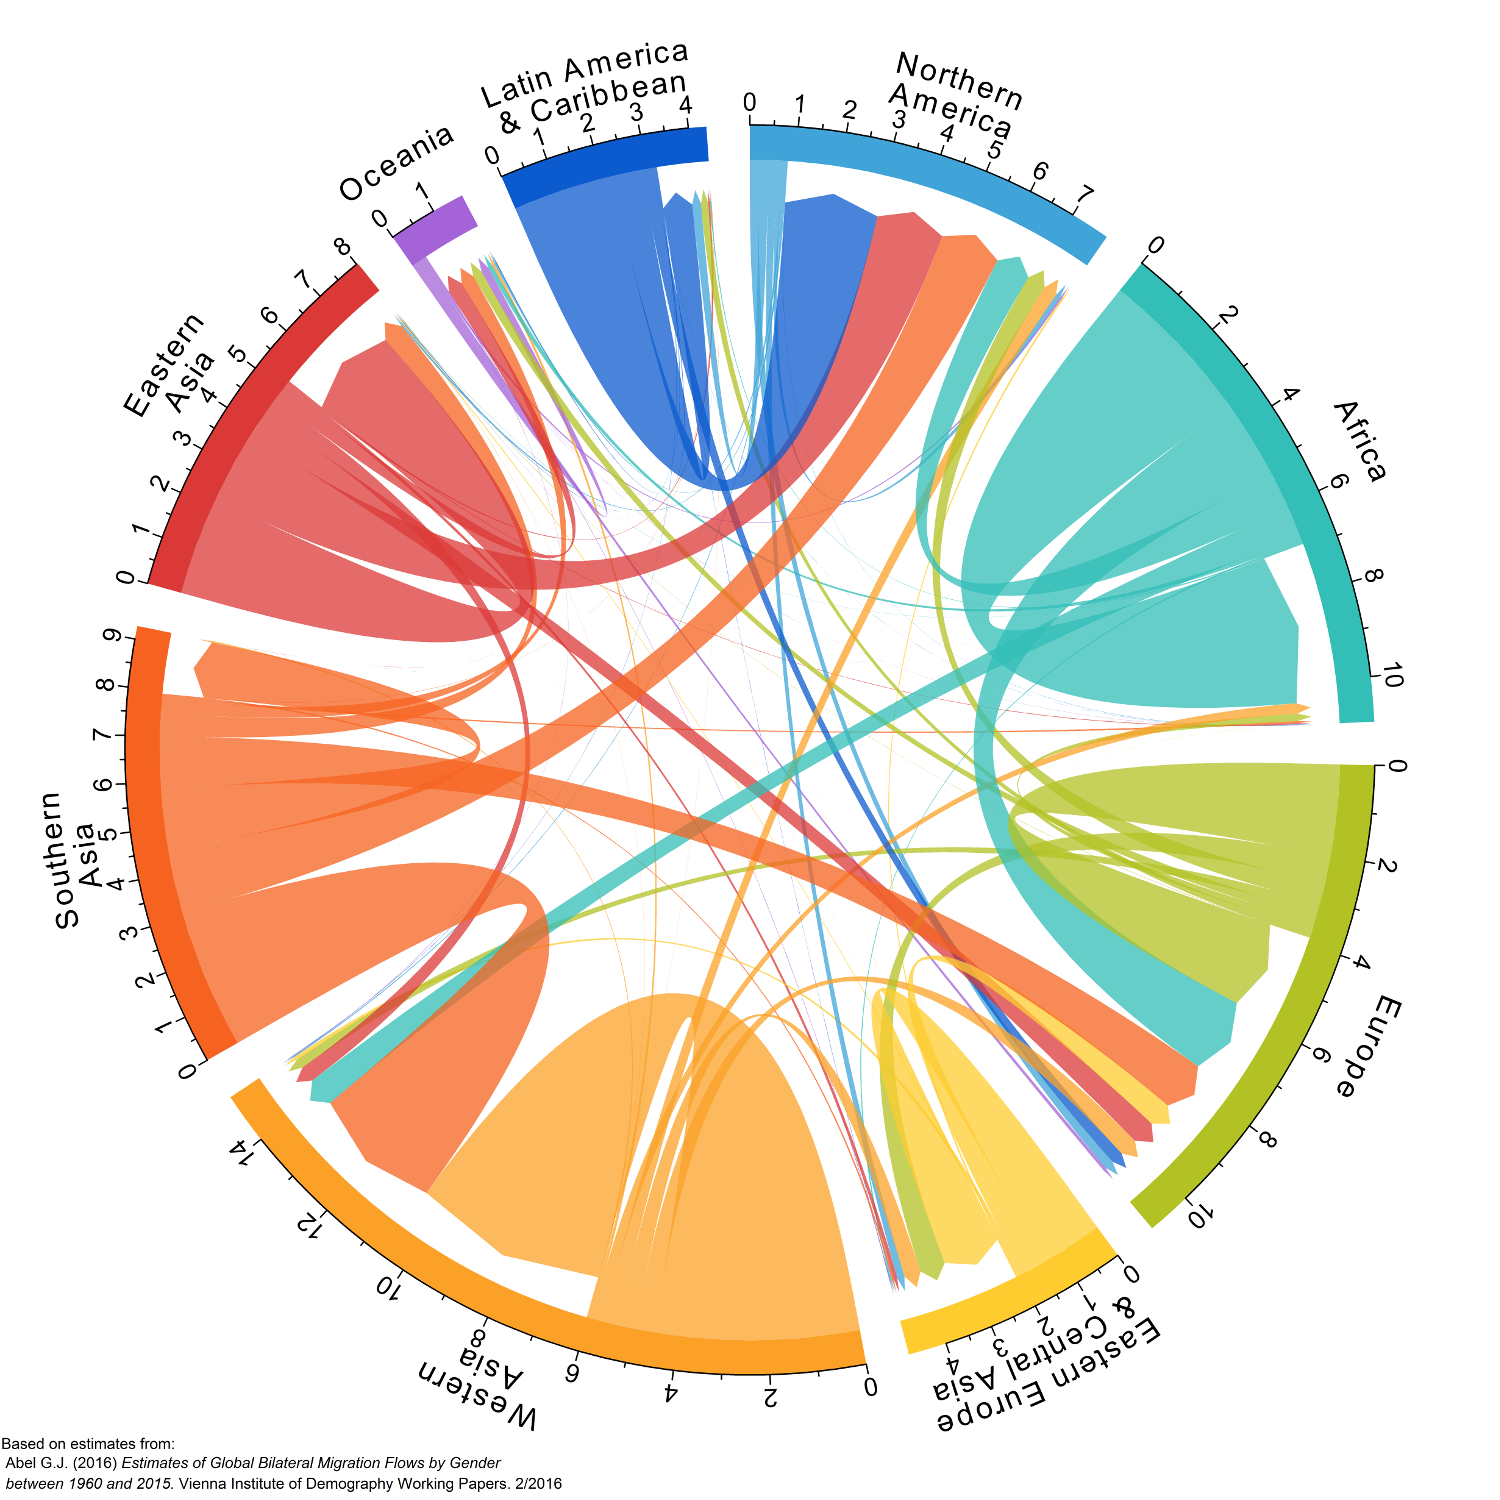
\includegraphics[scale=1.5]{migration}
  \end{figure}  
  \medskip
  \textbf{NB -} Largest migration flows between developing countries.
\end{frame}
%--------------------------------------

%--------------------------------------
\begin{frame}
  The USA is a popular destination country for migrants, specifically from Mexico
  \begin{itemize}
    \item One third of foreign-born US residents are Mexican
    \item 1 in 10 Mexicans end up living in the US
    \item 97\% of Mexican migrants go to US
  \end{itemize}
  \medskip
  Most migrants are low-skilled workers and much of Mexican-US migration is cyclical.
  In recent years there has been a decrease in migration
  \begin{enumerate}
    \item Enhanced border protection
    \item Recession decreased job prospects
  \end{enumerate}
\end{frame}
%--------------------------------------

%--------------------------------------
\begin{frame}
 \begin{figure}
   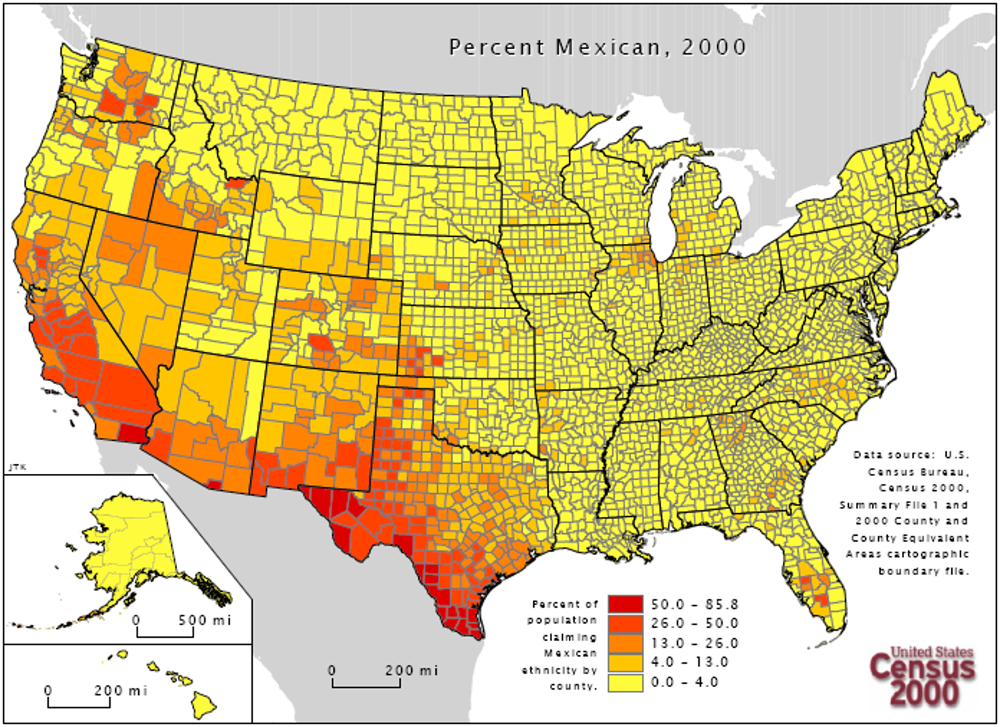
\includegraphics[scale=2]{Pctmexican.png}
 \end{figure}
\end{frame}
%--------------------------------------

%--------------------------------------
\begin{frame}{Most immigrants per country}\framesubtitle{source: Business Insider}
 \begin{figure}
   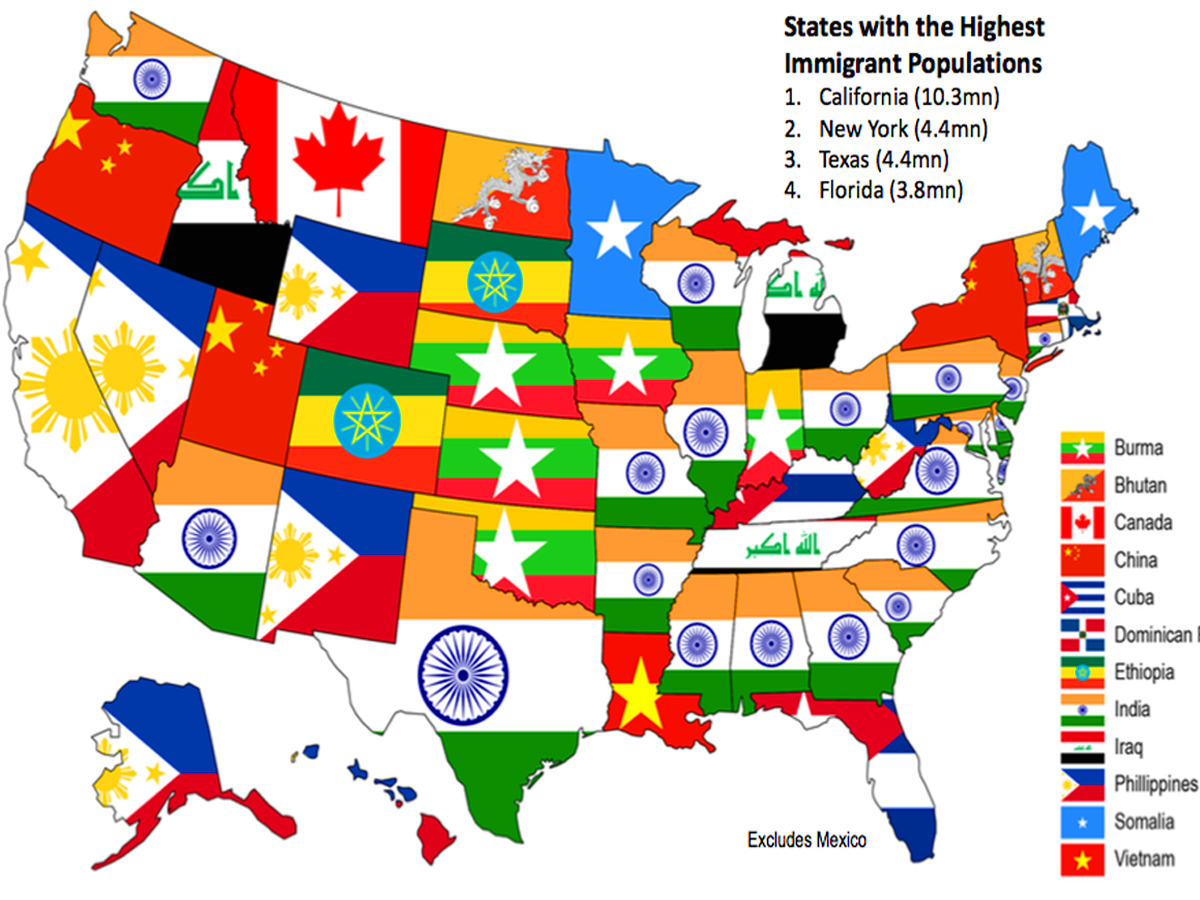
\includegraphics[scale=.2]{us_immigration2.png} 
 \end{figure}
\end{frame}
%--------------------------------------

%--------------------------------------
\begin{frame}{Immigration in Japan}
\framesubtitle{source: The Wall Street Journal}
  \begin{figure}
    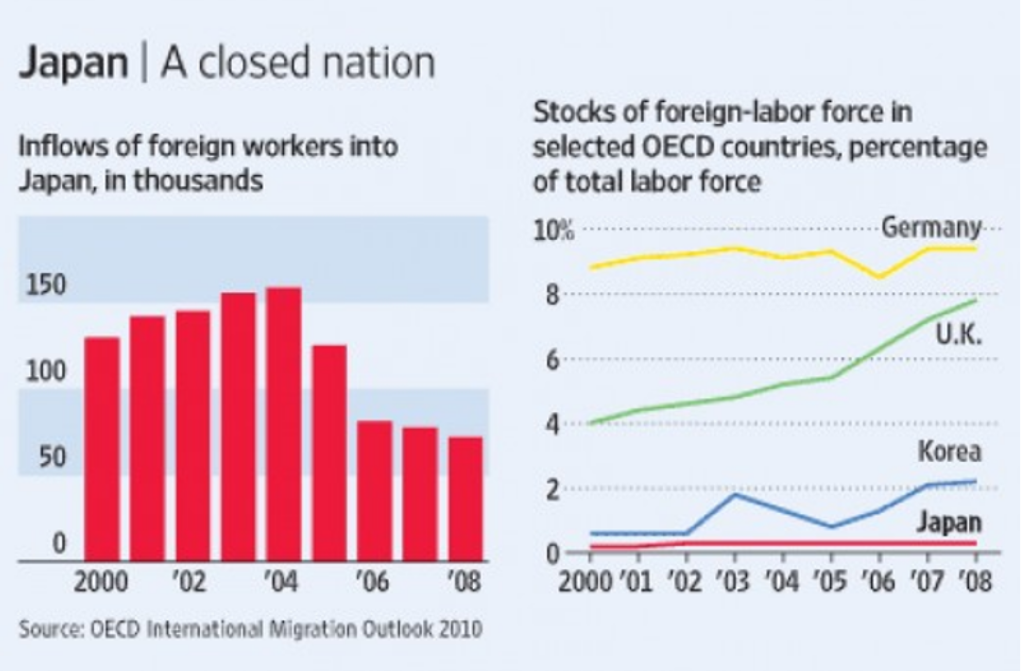
\includegraphics{jpn_migration}
  \end{figure}  
\end{frame}
%--------------------------------------

%--------------------------------------
\begin{frame}
Returning to the question about immigration to America: let's assume that their economy produces two goods
  \begin{itemize}
    \item clothing $C$ and food $F$
  \end{itemize}
  \medskip 
with three production factors
\begin{itemize}
  \item labour $L$, capital $K$, and land $T$  
\end{itemize}
\medskip
Each factor is paid the value of its marginal product.
 \begin{align*}
  r_c&=p_c\cdot MPK_c; r_f=p_f\cdot MPT_f\\
  w&=p_c\cdot MPL_c=p_f\cdot MPL_f
 \end{align*}
\medskip
While $K$ and $T$ are fixed, $L$ changes in response to shocks such as immigration.
\end{frame}
%--------------------------------------

%--------------------------------------
\begin{frame}{Labour allocation pre-immigration}
  \begin{figure}
    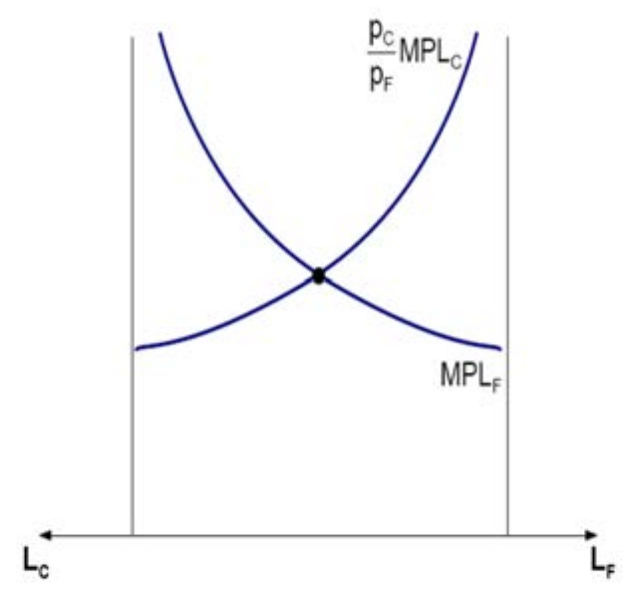
\includegraphics{labour1.png}
  \end{figure}
  $y$-axis is $\frac{w}{p_f} = MPL_f = \frac{p_c}{p_f}MPL_c$
\end{frame}
%--------------------------------------

%--------------------------------------
\begin{frame}{Effect of increase in labour endowment}
  \begin{figure}
    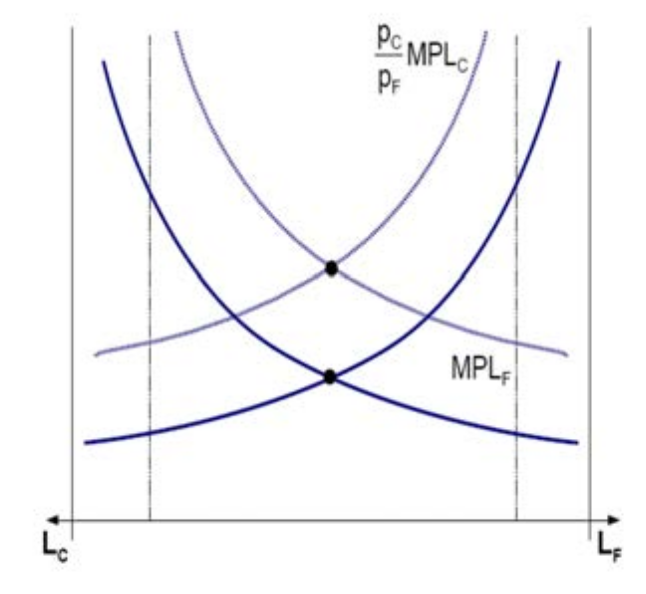
\includegraphics{labour2.png}
  \end{figure}
\end{frame}
%--------------------------------------

%--------------------------------------
\begin{frame}
 Following an increase in labour endowment, additional labour will go to both sectors.
 What will be the impact on worker's welfare?
 \begin{align*}
 MPL_c&=\frac{w}{p_c}\\
 MPL_f&=\frac{w}{p_f}
 \end{align*}
 \medskip
 Marginal productivity will decrease in both sectors due to labour increase: welfare falls.
\end{frame}
%--------------------------------------

%--------------------------------------
\begin{frame}
   What about the welfare of the capital owners?
 \begin{align*}
 MPK_c&=\frac{r_c}{p_c}\\
 MPT_f&=\frac{r_f}{p_f}
 \end{align*}
 At constant relative prices the returns to capital and land will increase in both sectors due to the labour increase: welfare increases
\end{frame}
%--------------------------------------

%--------------------------------------
\begin{frame}
 The specific factors model can help us understand why certain people are pro-trade while others are not. 
 Mayda \& Rodrik (2006) test this empirically using survey data and found that pro-trade preferences are correlated with
 \begin{itemize}
   \item Individual's level of human capital
   \item Trade exposure of the sector in which the individual works: non-traded sectors are more pro-trade   
 \end{itemize}
\end{frame}
%--------------------------------------

%--------------------------------------
\begin{frame}
  \begin{figure}
    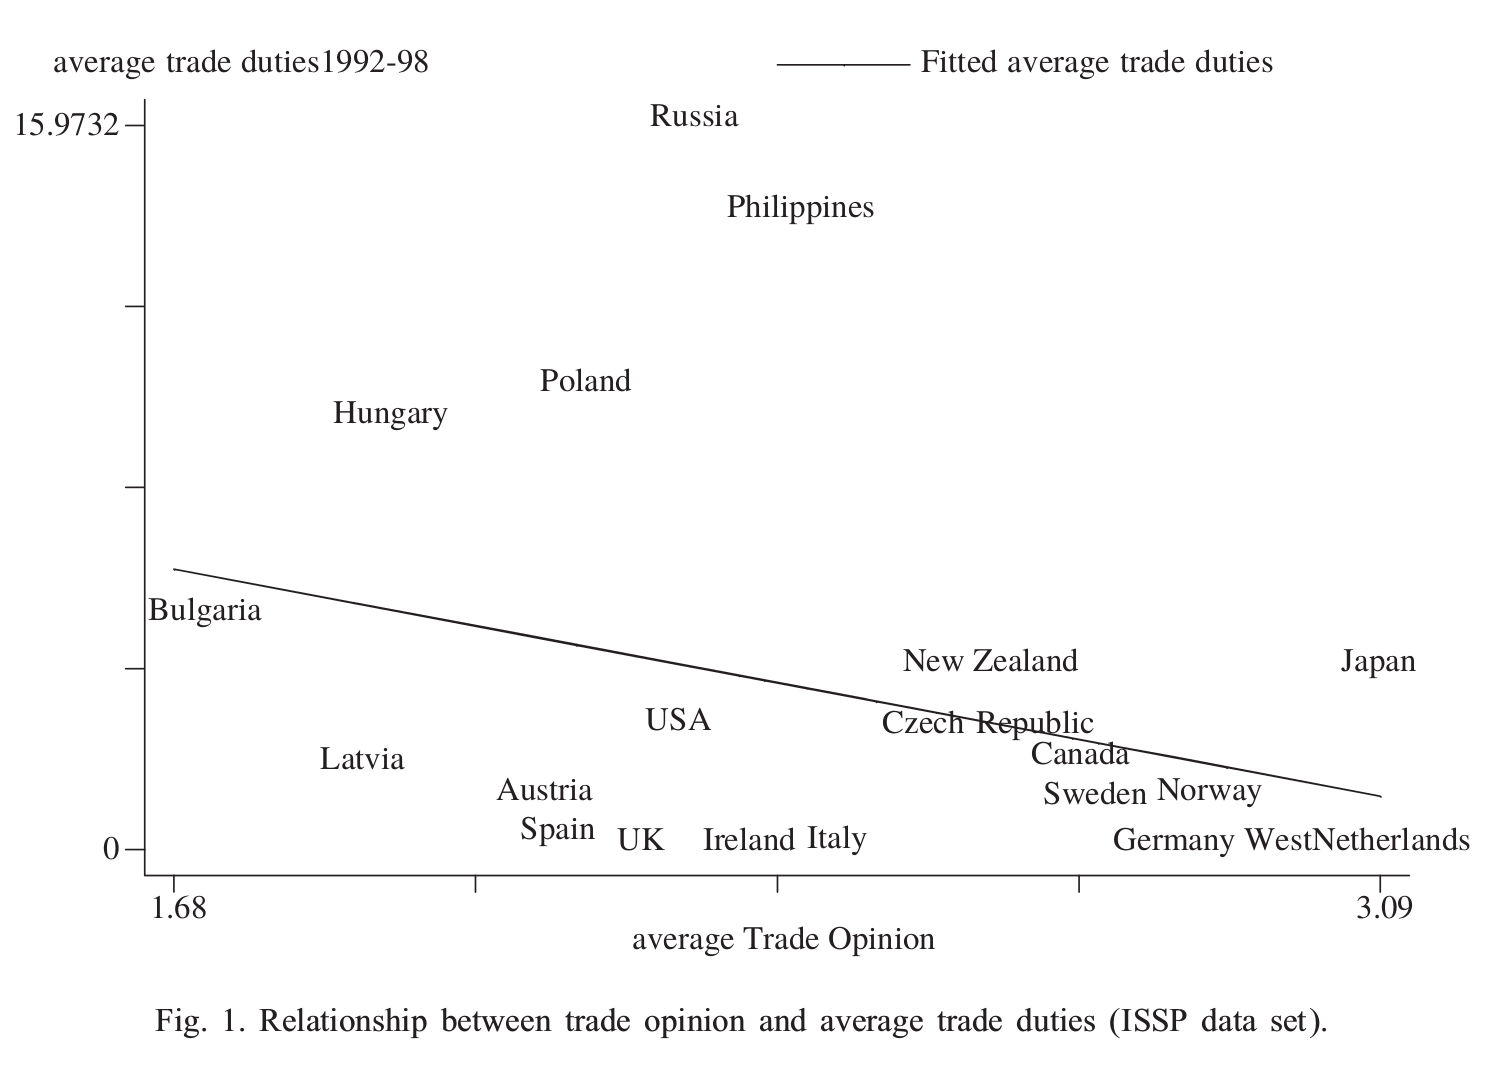
\includegraphics[scale=.7]{tradepreferences.png}
  \end{figure}
\end{frame}
%--------------------------------------

%--------------------------------------
\begin{frame}
 Summarising,in contrast with the Ricardian model the import-competing sector does not vanish in the specific-factors model when a country opens up to trade. 
 \begin{itemize}
  \item There is a strong effect of changes in relative prices on income distribution and welfare across sectors
 \end{itemize}
 \medskip
 Importantly, countries can share the same technologies and still benefit from trade
 \begin{itemize}
   \item Comparative advantage is driven by differences in factor abundance
   \item In Ricardian model there is no incentive for trade when they have the same technology
 \end{itemize}
\end{frame}
%--------------------------------------

%------------------------------------------------------------------------------
\end{document}
